%%
%% This is file `minimalexample',
%% generated with the docstrip utility.
%%
%% The original source files were:
%%
%% CASUS.dtx  (with options: `minimalexample')
%% ----------------:| --------------------------------------------------------
%% CASUS:           | Corporate Design for the CASUS project
%% Author:          | Tobias Schlemmer
%% E-mail:          | Tobias.Schlemmer@web.de
%% License:         | LaTeX files are released under the LaTeX Project Public License v1.3c or later
%%                  | Needed graphics files are not covered by this license.
%% See:             | http://www.latex-project.org/lppl.txt
%% 
\documentclass[english,aspectratio=169]{beamer}
\usepackage[utf8]{inputenc}
\usepackage[TS1,T1]{fontenc}
\usepackage{babel}
\usepackage{lmodern}
\usepackage{bm}
\usepackage{bbm}
\usepackage[framemethod=TikZ]{mdframed}

\usepackage[labelformat=empty,font=tiny,singlelinecheck=false]{caption}

\usepackage{mathtools}
\usepackage{multirow}
% Math notations are written in serif
\usefonttheme[onlymath]{serif}

\setbeamertemplate{navigation symbols}{}%remove navigation symbols

\usepackage{ragged2e}


\usepackage{pgfplots}

\pgfplotsset{compat=newest}
\usetikzlibrary{patterns}
\usepgfplotslibrary{fillbetween}

\let\tempone\itemize
\let\temptwo\enditemize
\renewenvironment{itemize}{\tempone\addtolength{\itemsep}{0.35\baselineskip}}{\temptwo}

\usepackage{xcolor}

\usetikzlibrary{positioning, matrix}
\newcommand{\myunit}{1 cm}
\tikzset{
    node style sp/.style={draw,circle,minimum size=\myunit},
    node style ge/.style={circle,minimum size=\myunit},
    arrow style mul/.style={draw,sloped,midway,fill=white},
    arrow style plus/.style={midway,sloped,fill=white},
}

% Bib
\usepackage[style=apa,backend=biber]{biblatex}
\addbibresource{bibliography.bib}
\renewcommand*{\bibfont}{\scriptsize}
\setbeamertemplate{bibliography item}{} % Remove icon from the list of references

% Argmin and argmax
\usepackage{amsmath}
\DeclareMathOperator*{\argmin}{arg\,min}
\DeclareMathOperator*{\argmax}{arg\,max}

% Left/right align figure
\usepackage[export]{adjustbox}

\renewcommand{\emph}[1]{\textcolor[HTML]{006d2c}{\fontseries{sb}\selectfont #1}}

\usetheme{CASUS}
\title[Practices of UQ in Engineering]{%
  Functional ANOVA and\protect\\
  Variance Decomposition of Functions
}
%\subtitle{}
\author{Damar Wicaksono}

\def\blfootnote{\xdef\@thefnmark{}\@footnotetext}

%%%%%%%%%%%%%%%%%%%%%%%%%%%%%%%%%%%%%%%%%%%%%%%%%%%%%%%%%%%%%%%%%%%%%%%%%%%%%%
% \embedvideo{<poster or text>}{<video file (MP4+H264)>}
%%%%%%%%%%%%%%%%%%%%%%%%%%%%%%%%%%%%%%%%%%%%%%%%%%%%%%%%%%%%%%%%%%%%%%%%%%%%%%
\usepackage[bigfiles]{pdfbase}
\ExplSyntaxOn
%%begin novalidate
\cs_new:Npn\embedvideo#1#2{
%%end novalidate
  \leavevmode
  \pbs_pdfobj:nnn{}{fstream}{{}{#2}}
  \pbs_pdfobj:nnn{}{dict}{
    /Type/Filespec/F~(#2)/UF~(#2)
    /EF~<</F~\pbs_pdflastobj:>>
  }
  \tl_set:Nx\video{\pbs_pdflastobj:}%
  %
  \pbs_pdfobj:nnn{}{dict}{
    /Type/RichMediaInstance/Subtype/Video
    /Asset~\video
    /Params~<</Binding/Foreground>>
  }
  %
  \pbs_pdfobj:nnn{}{dict}{
    /Type/RichMediaConfiguration/Subtype/Video
    /Instances~[\pbs_pdflastobj:]
  }
  %
  \pbs_pdfobj:nnn{}{dict}{
    /Type/RichMediaContent
    /Assets~<<
      /Names~[(#2)~\video]
    >>
    /Configurations~[\pbs_pdflastobj:]
  }
  \tl_set:Nx\rmcontent{\pbs_pdflastobj:}%
  %
  \pbs_pdfobj:nnn{}{dict}{
    /Activation~<<
      /Condition/XA
      /Presentation~<<
        /Transparent~true
        /Style/Embedded
        /PassContextClick~true
      >>
    >>
    /Deactivation~<</Condition/PC>>
  }
  %
  \hbox_set:Nn\l_tmpa_box{#1}
  \tl_set:Nx\l_box_wd_tl{\dim_use:N\box_wd:N\l_tmpa_box}
  \tl_set:Nx\l_box_ht_tl{\dim_use:N\box_ht:N\l_tmpa_box}
  \tl_set:Nx\l_box_dp_tl{\dim_use:N\box_dp:N\l_tmpa_box}
  \pbs_pdfxform:nnnnn{1}{1}{}{}{\l_tmpa_box}
  %
  \pbs_pdfannot:nnnn{\l_box_wd_tl}{\l_box_ht_tl}{\l_box_dp_tl}{
    /Subtype/RichMedia
    /BS~<</W~0/S/S>>
    /Contents~(embedded~video~file:#2)
    /NM~(rma:#2)
    /AP~<</N~\pbs_pdflastxform:>>
    /RichMediaSettings~\pbs_pdflastobj:
    /RichMediaContent~\rmcontent
  }
  \phantom{#1}
}%
\ExplSyntaxOff
%%%%%%%%%%%%%%%%%%%%%%%%%%%%%%%%%%%%%%%%%%%%%%%%%%%%%%%%%%%%%%%%%%%%%%%%%%%%%%

\begin{document}
\titleframe
\contentsframe

%%%%%%%%%%%%%%%%%%%%%%%%%%%%%%%%%%%%%%%%%%%%%%%%%%
\section{Functional Decomposition}
%%%%%%%%%%%%%%%%%%%%%%%%%%%%%%%%%%%%%%%%%%%%%%%%%%

%=============================================================================
\begin{frame}[fragile]{Functional Decomposition}
\small

\vspace{-2.0em}

\begin{exampleblock}{}
  \emph{Functional decomposition} is a method that:
  \vspace{1.0em}
  \begin{itemize}
    \item \emph{breaks down} complex multidimensional functions, and
    \item \emph{represents} them as the sum of \emph{individual effects} (also called \emph{main effects})
          of the inputs and the \emph{interaction effects} between them.
  \end{itemize}
  \vspace{0.5em}
  It provides a way to look and succinctly describe complex multidimensional functions.
\end{exampleblock}

\vspace{1.5em}

\begin{onlyenv}<2>
  \small
  Let $f: \mathbb{R}^m \rightarrow \mathbb{R}$, then functional decomposition of $f$ yields:
  \vspace{0.5em}
  \begin{equation*}
    f(\boldsymbol{x}) = \underbrace{f_0}_{\text{\tiny baseline effect}} + \underbrace{f_1(x_1) + f_2 (x_2) + \ldots}_{\text{\tiny main effects}} + \underbrace{f_{1, 2}(x_1, x_2) + f_{1, 3} (x_1, x_3) + \ldots}_{\text{\tiny $2$-way interaction effects}} + \ldots + \underbrace{f_{1, \ldots, m} (x_1, \ldots, x_m)}_{\text{\tiny $m$-way interaction effect}}
  \end{equation*}
  \vspace{0.5em}
\end{onlyenv}

\begin{onlyenv}<3>
  \small
  Let $f: \mathbb{R}^m \rightarrow \mathbb{R}$, then functional decomposition of $f$ yields:
  \vspace{0.5em}
  \begin{equation*}
    f(\boldsymbol{x}) = \underbrace{f_0}_{\text{\tiny baseline effect}} + \underbrace{f_1(x_1) + f_2 (x_2) + \ldots}_{\text{\tiny main effects}} + \underbrace{f_{1, 2}(x_1, x_2) + f_{1, 3} (x_1, x_3) + \ldots}_{\text{\tiny $2$-way interaction effects}} + \ldots + \underbrace{f_{1, \ldots, m} (x_1, \ldots, x_m)}_{\text{\tiny $m$-way interaction effect}}
  \end{equation*}
  \vspace{0.5em}
  Observations:
  \begin{itemize}
    \item There are $2^m$ components in the summation
    \item The summation recovers the original function
  \end{itemize}
\end{onlyenv}

\end{frame}

%=============================================================================
\begin{frame}[fragile]{Example}
\small

\vspace{-1.0em}

Consider a two-dimensional function:

\begin{equation*}
  f(x_1, x_2) = \frac{1}{6} \left[ 120 + 20 x_1 \sin{(5x_1) + 30 e^{-5 x_2} + 20 x_1 \sin{(5 x_1)} e^{-5 x_2} - 100 } \right],\;\; x_1, x_2 \in [0, 1].
\end{equation*}
{\hfill \raggedright \tiny \textcolor{blue}{(\cite{Lim2002})}}

\vspace{-0.5em}

\begin{figure}
  \centering
  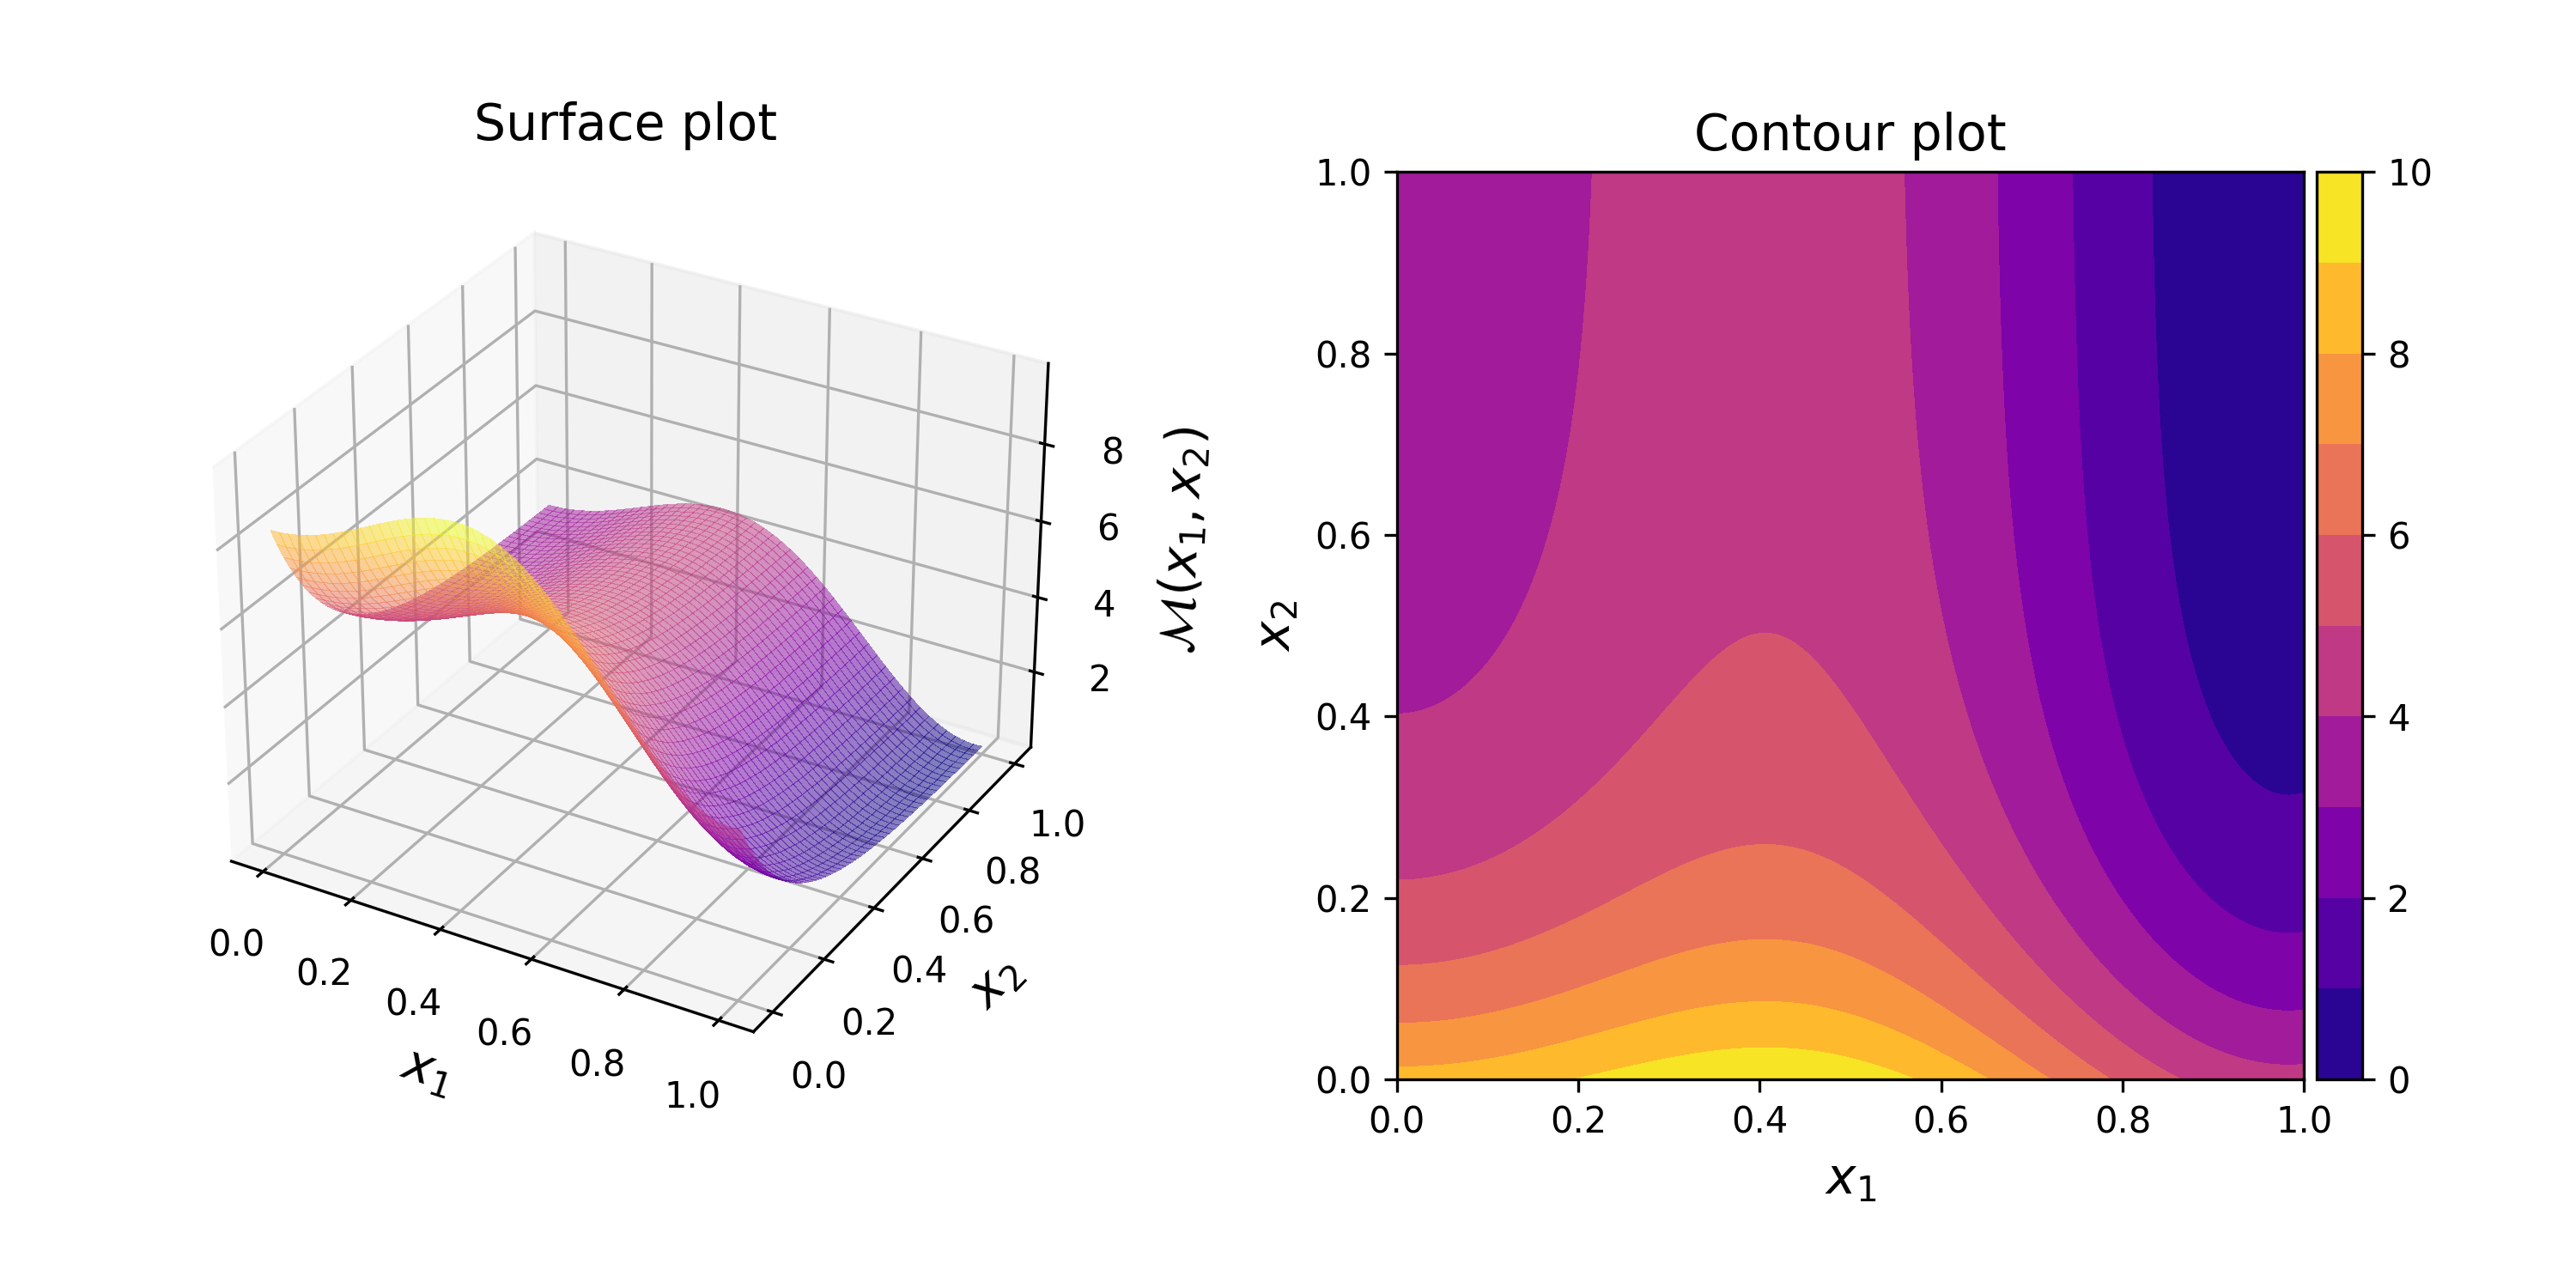
\includegraphics[width=0.7\textwidth]{./figures/lim2d.png}
\end{figure}

\end{frame}

%=============================================================================
\begin{frame}[fragile]{Example: Functional Decomposition}
\small
We have the two following constraints of our decomposition:
\vspace{1.0em}
\begin{itemize}
\item There are $2^m$ components in the summation
\item The summation recovers the original function
\end{itemize}

\vspace{1.5em}

\begin{onlyenv}<2-3>
  So, by \emph{inspection}:
  \begin{equation*}
    f(x_1, x_2) = \frac{1}{6} \left[ 120 + 20 x_1 \sin{(5x_1) + 30 e^{-5 x_2} + 20 x_1 \sin{(5 x_1)} e^{-5 x_2} - 100 } \right],
  \end{equation*}
  \begin{eqnarray*}
    f_0 = \frac{20}{6}; \; f_1(x_1) = \frac{20}{6} x_1 \sin{(5 x_1)}; \;  f_2(x_2) = 5 e^{-5 x_2}; \; f_{1, 2}(x_1, x_2) = x_1 \sin{(5 x_1)} e^{-5 x_2}.
  \end{eqnarray*}
  There are $2^2 = 4$ components by just looking and the sum indeed recovers the original function.
\end{onlyenv}

\vspace{-0.6em}

\begin{exampleblock}<3>{}
  \centering
  Are we done?
\end{exampleblock}

\end{frame}

%=============================================================================
\begin{frame}[fragile]{Problems}
\small

Our way of decomposing the function by inspection is unsatisfying:
\vspace{1.5em}
\begin{onlyenv}<1-4>
\begin{itemize}
  \item<2-4> \emph{Black-box functions}: \textit{What if you can't see the formula?}
  \item<3-4> \emph{Uniqueness}: You can come with different decompositions as long as the sum recovers the function by adjusting the last term.\\
  \vspace{1.0em}
  Example:
  \begin{equation*}
    f_1(x_1) = \frac{20}{6} \left( x_1 \sin{(5 x_1)} + x_1 \cos{(5 x_1)} \right); \; f_{1, 2}(x_1, x_2) = x_1 \left( \sin{(5 x_1)} - \frac{20}{6} \cos{(5 x_1)} \right) e^{-5 x_2}.
  \end{equation*}

  \item<4-4> \emph{Input effect}: \textit{Shouldn't the decomposition take into account the inputs?}\\
  \vspace{1.0em}
  Example:
  \begin{equation*}
    x_2 \in [3, 4] \rightarrow f_2 \approx 0, f_{1, 2} \approx 0.
  \end{equation*}
  \vspace{1.0em}
  The effect of $x_2$ on $f$ depends how it is specified.

\end{itemize}
\end{onlyenv}

\begin{exampleblock}<5>{}
  \centering
  \emph{Our decomposition is neither unique nor meaningful.}
\end{exampleblock}

\end{frame}

%%%%%%%%%%%%%%%%%%%%%%%%%%%%%%%%%%%%%%%%%%%%%%%%%%
\section{Functional ANOVA}
%%%%%%%%%%%%%%%%%%%%%%%%%%%%%%%%%%%%%%%%%%%%%%%%%%

%=============================================================================
\begin{frame}{Outline}
  \tableofcontents[currentsection]
\end{frame}

%==============================================================================
\begin{frame}[fragile]{Assumption: Space of square-integrable functions}
\small

We assume that our function of interest belongs
to $L^2(\mathcal{D}_{\boldsymbol{X}}, \rho_{\boldsymbol{X}})$, i.e., the space of square-integrable functions
over domain $\mathcal{D}_{\boldsymbol{X}} \subseteq \mathbb{R}^m$ with respect to the weight function $\rho_{\boldsymbol{X}}$.

\vspace{1.5em}

\begin{onlyenv}<1>  
\begin{itemize}
  \item A function $f$ is square integrable over the domain $\mathcal{D}_{\boldsymbol{X}}$ with respect to the weight function $\rho_{\boldsymbol{X}}$ if:
  \begin{equation*}
    \int_{\mathcal{D}_{\boldsymbol{X}}} f^2 (\boldsymbol{x}) \rho_{\boldsymbol{X}}(\boldsymbol{x}) \; d\boldsymbol{x} < \infty.
  \end{equation*}
  \item The space is equipped with inner product (it's a Hilbert space). That is, for $f, g \in L^2(\mathcal{D}_{\boldsymbol{X}}, \rho_{\boldsymbol{X}})$,
    \begin{equation*}
      \langle f, g \rangle_{\rho_{\bm{X}}} \equiv \int_{\mathcal{D}_{\bm{X}}} f(\bm{x}) g(\bm{x}) \rho_{\bm{X}}(\bm{x}) d\bm{x}.
    \end{equation*}
  \item The function norm is defined as:
  \begin{equation*}
    \lVert f \rVert^2_{\rho_{\bm{X}}} \equiv \langle f, f \rangle_{\rho_{\bm{X}}} < \infty.
  \end{equation*} 
\end{itemize}
\end{onlyenv}

\begin{exampleblock}<2>{}
  In practice, we are interested in selecting the weight function $\rho_{\boldsymbol{X}}$
  to be a \emph{(joint) probability density function}.

  \vspace{0.5em}

  $L^2(\mathcal{D}_{\boldsymbol{X}}, \rho_{\boldsymbol{X}})$ is then equivalent to
  the space of random variables with \emph{finite variance},
  where the elements are functions of random vectors.
\end{exampleblock}

\end{frame}


%==============================================================================
\begin{frame}[fragile]{Uncertainty Quantification Framework}
\small

\vspace{-1.5em}

\begin{exampleblock}{}
  In practice, we are interested in selecting the weight function $\rho_{\boldsymbol{X}}$
  to be a \emph{(joint) probability density function}.

  \vspace{0.5em}

  $L^2(\mathcal{D}_{\boldsymbol{X}}, \rho_{\boldsymbol{X}})$ is then equivalent to
  the space of random variables with \emph{finite variance},
  where the elements are functions of random vectors.
\end{exampleblock}

\begin{figure}
  \centering
  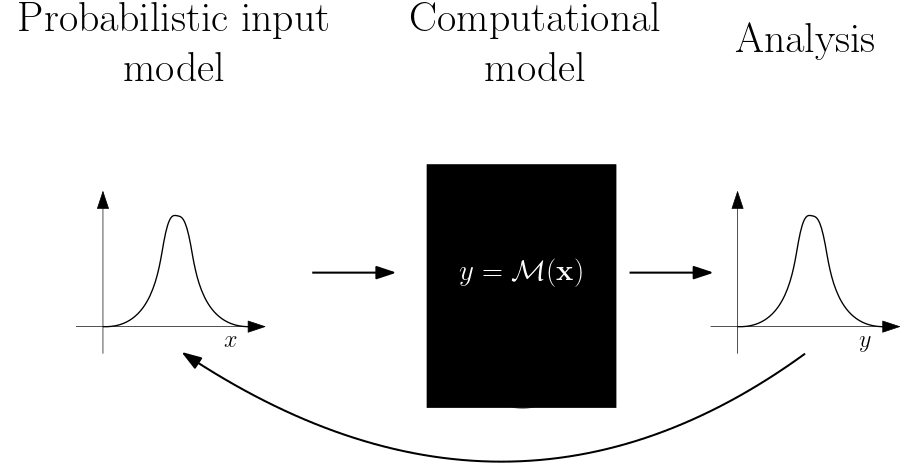
\includegraphics[width=0.6\textwidth]{./figures/uq_framework_blackbox}
\end{figure}

\vspace{-2.0em}

{\hfill \raggedright \tiny adapted from \textcolor{blue}{(\cite{Marelli2014})}}
\end{frame}

%==============================================================================
\begin{frame}[fragile]{Assumption: Mutually Independent $\bm{X}$}
\small

We further assume that $\bm{X}$ is a mutually independent random vector
such that its joint probability density function (PDF) reads:

\begin{equation*}
  \rho_{\bm{X}}(\bm{x}) = \prod_{j = 1}^m \rho_{X_j} (x_j),
\end{equation*}

where $\rho_{X_j}$ is the univariate PDF of $X_j$.

\end{frame}

%==============================================================================
\begin{frame}[fragile]{Multi-Index Notation}
\small

Through decomposition, we write an $m$-dimensional function $f$ as a sum of functions:
\begin{equation*}
  f(\bm{x}) = \sum_{\bm{u} \subseteq [1: m]} f_{\bm{u}} (\bm{x}_{\bm{u}}),
\end{equation*}
\begin{onlyenv}<1>
  where:
  \vspace{1.0em}
  \begin{itemize}
    \item $[1:m]$ is a short-hand for the set $\{ 1, \ldots, m\}$
    \item $\bm{x}_{\bm{u}}$ is the vector of inputs in the index set $\bm{u}$,
          i.e., $\bm{u} = \{ i_1, \ldots, i_{\lvert \bm{u} \rvert} \}$ means
          $(x_i)_{i \in \bm{u}}$
    \item $f_{\bm{u}}$ is the component function that depends only on $\bm{x}_{\bm{u}}$
  \end{itemize}

\end{onlyenv}

\begin{onlyenv}<2>
  \emph{Example}: For $m = 3$, the full decomposition of $f$ consists of $2^3 = 8$ terms and it reads:
  \begin{align*}
    f(\bm{x}) & = f_\emptyset & \text{\footnotesize baseline effect} \\
              &\quad + f_{\{1\}} (x_1) + f_{\{2\}} (x_2) + f_{\{3\}} (x_3) & \text{\footnotesize main effects} \\
              &\quad + f_{\{1, 2\}} (x_1, x_2) + f_{\{1, 3\}} (x_1, x_3) + f_{\{2, 3\}} (x_2, x_3) & \text{\footnotesize $2$-way interactions} \\
              &\quad + f_{\{1, 2, 3\}} (x_1, x_2, x_3). & \text{\footnotesize $3$-way interactions}
  \end{align*}
\end{onlyenv}

\end{frame}

%==============================================================================
\begin{frame}[fragile]{Functional ANOVA: Constructive Definition}
\small

We seek to obtain a unique functional decomposition of $f$ using the following \emph{summands}:
\vspace{1.0em}
\begin{itemize}
  \item<1-> \emph{Baseline effect} for $\bm{u} = \emptyset$ (global mean)
  \begin{equation*}
    f_\emptyset = \int_{\mathcal{D}_{\bm{X}}} f(\bm{x}) \rho_{\bm{X}} (\bm{x}) \; d\bm{x}.  
  \end{equation*}
  
  \item<2-> \emph{Main effect} for $\bm{u} = \{ j \}, j = 1, \ldots, m$ (singletons)
  \begin{equation*}
    f_{\{ j \}} (x_j) = \int_{\mathcal{D}_{\bm{X}_{\sim{\{ j \}}}}} f (\bm{x}) \rho_{\bm{X}_{\sim \{j\}}} (\bm{x}_{\sim \{j\}}) \; d\bm{x}_{\sim \{j\}} - f_\emptyset
  \end{equation*}

  \item<3-> \emph{Interaction effect} for $\bm{u} \subseteq [1:m]$, $\bm{u} \neq \emptyset, \lvert \bm{u} \rvert > 1$
  \begin{equation*}
    f_{\bm{u}} (x_{\bm{u}}) = \int_{\mathcal{D}_{\bm{X}_{\sim \bm{u}}}} f (\bm{x}) \rho_{\bm{X}_{\sim \bm{u}}} (\bm{x}_{\sim \bm{u}}) \; d\bm{x}_{\sim \bm{u}} - \sum_{\bm{v} \subset \bm{u}} f_{\bm{v}} (\bm{x}_{\bm{v}})
  \end{equation*}
\end{itemize}

where $\sim \bm{u}$ is the set complement of $\bm{u}$.

\end{frame}

%==============================================================================
\begin{frame}[fragile]{Functional ANOVA: Intuition}
\small

Consider the \emph{interaction effect} for $\bm{u} \subseteq [1:m]$, $\bm{u} \neq \emptyset, \lvert \bm{u} \rvert > 1$
\begin{equation*}
  f_{\bm{u}} (x_{\bm{u}}) = \int_{\mathcal{D}_{\bm{X}_{\sim \bm{u}}}} f (\bm{x}) \rho_{\bm{X}_{\sim \bm{u}}} (\bm{x}_{\sim \bm{u}}) \; d\bm{x}_{\sim \bm{u}} - \sum_{\bm{v} \subset \bm{u}} f_{\bm{v}} (\bm{x}_{\bm{v}})
\end{equation*}

\begin{block}{Intuition}
  When we compute $f_{\bm{u}}$:
  \vspace{0.5em}
  \begin{itemize}
    \item We don't want to attribute anything to it that can be explained by $\bm{x}_{\bm{v}}$ for $\bm{v} \subset \bm{u}$
    \item $f_{\bm{u}}$ must be strictly only due to $\bm{x}_{\bm{u}}$;
          \emph{not} $\bm{x}_{\sim \bm{u}}$ \emph{nor} subsets of $\bm{x}_{\bm{u}}$ (lower order terms)
    \item Therefore, we integrate $f$ over all $\bm{x}_{\sim \bm{u}}$ then substract all the lower order terms
  \end{itemize}
\end{block}

\end{frame}

%==============================================================================
\begin{frame}[fragile]{Functional ANOVA: Example}
\small

\vspace{-1em}

Consider $f \in L^2(\mathcal{D}_{\boldsymbol{X}}, \rho_{\boldsymbol{X}})$ with mutually independent $\bm{X}$ for $m = 3$:
\vspace{1.0em}
\begin{itemize}
  \item \emph{Baseline effect} (global mean)
  \begin{equation*}
    f_\emptyset = \int_{\mathcal{D}_{X_1}} \int_{\mathcal{D}_{X_2}} \int_{\mathcal{D}_{X_3}} f(\bm{x}) \rho_{X_1} (x_1) \rho_{X_2} (x_2) \rho_{X_3} (x_3) \; dx_1 dx_2 dx_3.
  \end{equation*}
  
  \item \emph{Main effects}
  \begin{align*}
    f_{\{ 1 \}} (x_1) & = \int_{\mathcal{D}_{X_2}} \int_{\mathcal{D}_{X_3}} f (\bm{x}) \rho_{X_2} (x_2) \rho_{X_3} (x_3) \; dx_2 dx_3 - f_\emptyset \\
    f_{\{ 2 \}} (x_2) & = \int_{\mathcal{D}_{X_1}} \int_{\mathcal{D}_{X_3}} f (\bm{x}) \rho_{X_1} (x_1) \rho_{X_3} (x_3) \; dx_1 dx_3 - f_\emptyset \\
    f_{\{ 3 \}} (x_3) & = \int_{\mathcal{D}_{X_1}} \int_{\mathcal{D}_{X_2}} f (\bm{x}) \rho_{X_1} (x_1) \rho_{X_2} (x_2) \; dx_1 dx_2 - f_\emptyset.
  \end{align*}

\end{itemize}

\end{frame}

%==============================================================================
\begin{frame}[fragile]{Functional ANOVA: Example}
\small

\vspace{-1em}

Consider $f \in L^2(\mathcal{D}_{\boldsymbol{X}}, \rho_{\boldsymbol{X}})$ for $m = 3$:
\vspace{1.0em}
\begin{itemize}  
  \item \emph{Two-way interaction effects}
  \begin{align*}
    f_{\{ 1, 2 \}} (x_1, x_2) & = \int_{\mathcal{D}_{X_3}} f (\bm{x}) \rho_{X_3} (x_3) \; dx_3 - f_{\{ 1 \}} (x_1) - f_{\{ 2 \}} (x_2) - f_\emptyset \\
    f_{\{ 1, 3 \}} (x_1, x_3) & = \int_{\mathcal{D}_{X_2}} f (\bm{x}) \rho_{X_2} (x_2) \; dx_2 - f_{\{ 1 \}} (x_1) - f_{\{ 3 \}} (x_2) - f_\emptyset \\
    f_{\{ 2, 3 \}} (x_2, x_3) & = \int_{\mathcal{D}_{X_1}} f (\bm{x}) \rho_{X_1} (x_1) \; dx_1 - f_{\{ 2 \}} (x_2) - f_{\{ 3 \}} (x_2) - f_\emptyset \\
  \end{align*}

  \item \emph{Three-way interaction effect}
  \begin{align*}
    f_{\{ 1, 2, 3 \}} (x_1, x_2, x_3)  & = f(\bm{x}) - f_{\{ 1, 2 \}} (x_1, x_2) - f_{\{ 1, 3 \}} (x_1, x_3) - f_{\{ 2, 3 \}} (x_2, x_3) \\
                                       &\quad - f_{\{ 1 \}} (x_1) - f_{\{ 2 \}} (x_2) - f_{\{ 3 \}} (x_3) - f_\emptyset
  \end{align*}

\end{itemize}

\end{frame}

%==============================================================================
\begin{frame}[fragile]{Functional ANOVA: Important Properties}
\small

Let $f \in L^2(\mathcal{D}_{\boldsymbol{X}} \subseteq \mathbb{R}^m, \rho_{\boldsymbol{X}})$ with mutually independent $\bm{X}$ such that its functional ANOVA decomposition:
\begin{equation*}
  f(\bm{x}) = \sum_{\bm{u} \subseteq [1: m]} f_{\bm{u}} (\bm{x}_{\bm{u}})
\end{equation*}

Then for $\bm{u}, \bm{v} \subseteq [1:m] \setminus \emptyset$:
\vspace{0.5em}
\begin{itemize}
  \item \emph{Lemma}: Functional ANOVA summands average to zero w.r.t any of its indices
  \begin{equation*}
    \int_{\mathcal{D}_{X_j}} f_{\bm{u}} (\bm{x}_{\bm{u}}) \rho_{X_j} (x_j) \; dx_j = 0,\;\; \forall j \in \bm{u}.
  \end{equation*}
  \item \emph{Lemma}: Functional ANOVA summands are orthogonal
  \begin{equation*}
    \int_{\mathcal{D}_{\bm{X}}} f_{\bm{u}} (\bm{x}_{\bm{u}}) \; f_{\bm{v}} (\bm{x}_{\bm{v}}) \; \rho_{\bm{X}} (\bm{x}) \; d\bm{x} = 0, \bm{u} \neq \bm{v}.
  \end{equation*}
\end{itemize}

\end{frame}

%==============================================================================
\begin{frame}[fragile]{Functional ANOVA: Variance Decomposition}
\small
\vspace{-1em}
\emph{ANOVA} stands for \emph{An}alysis \emph{o}f \emph{Va}riance; so taking it one step further.
\vspace{0.5em}
\begin{itemize}
  \item \emph{Total variance} of $f$
  \begin{equation*}
    \sigma^2 \equiv \int_{\mathcal{D}_{\bm{X}}} \left( f_{\bm{x}} (\bm{x}) - f_\emptyset \right)^2 \rho_{\bm{X}} (\bm{x}) \; d\bm{x}.
  \end{equation*}
  \item \emph{Partial variances} of $f_{\bm{u}}$
  \begin{equation*}
    \sigma_{\bm{u}}^2 \equiv \begin{cases}
      \int_{\mathcal{D}_{\bm{X}_{\bm{u}}}} f^2_{\bm{u}} (\bm{x}_{\bm{u}}) \rho_{\boldsymbol{X}_{\bm{u}}} (\bm{x}_{\bm{u}}) \; d\bm{x}_{\bm{u}}, & \lvert \bm{u} \rvert > 0 \\
      0, & \lvert \bm{u} \rvert = 0.     
    \end{cases}
  \end{equation*}
\end{itemize}
\begin{block}<2>{Theorem: Variance decomposition of $f$ (Sobol' decomposition)}
The total variance of $f$ is decomposed into  a sum of variances of the summands:
\begin{equation*}
  \sigma^2 = \sum_{\lvert \bm{u} \rvert > 0} \sigma_{\bm{u}}^2.
\end{equation*}
\end{block}
\end{frame}

%==============================================================================
\begin{frame}[fragile]{Functional ANOVA: Historical Perspective}
\small

\begin{columns}[T,onlytextwidth]
  \begin{column}{0.60\textwidth}

  (Functional) ANOVA has a long history rooted in statistics and applied mathematics:
  \vspace{0.5em}
  \begin{itemize}
    \item ANOVA for tabular data developed by Fisher \\
    {\hfill \raggedright \tiny \textcolor{blue}{(\cite{Fisher1919})}}
    \item generalized for $[0, 1]^m$ as U-statistics \\
    {\hfill \raggedright \tiny \textcolor{blue}{(\cite{Hoeffding1948})}}
    \item generalized for $[0, 1]^m$ as Sobol' decomposition for Quasi Monte Carlo integration \\
    {\hfill \raggedright \tiny \textcolor{blue}{(\cite{Sobol1969})}}
    \item popularized for practical sensitivity analysis in applied science and engineering\\
    {\hfill \raggedright \tiny \textcolor{blue}{(\cite{Saltelli2000})}}
    \item revisited in the context of Monte Carlo integration and effective dimensions\\
    {\hfill \raggedright \tiny \textcolor{blue}{(\cite{Caflisch1997,Liu2006})}}
  \end{itemize}
  \end{column}
  \begin{column}{0.40\textwidth}
    \begin{figure}[ht] 
      \begin{minipage}[b]{0.3\linewidth}
        \centering
        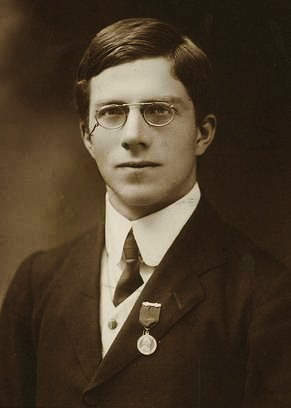
\includegraphics[height=.3\textheight]{./figures/fisher}\par 
        {\tiny R.A. Fisher \\ (1890--1962)}
        \vspace{0.7ex}
      \end{minipage}%%
      \begin{minipage}[b]{0.3\linewidth}
        \centering
        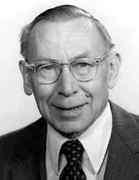
\includegraphics[height=.3\textheight]{./figures/hoeffding.jpg}\par 
        {\tiny W. Hoeffding \\ (1914--1991)}
        \vspace{0.7ex}
      \end{minipage}%%
      \begin{minipage}[b]{0.3\linewidth}
        \centering
        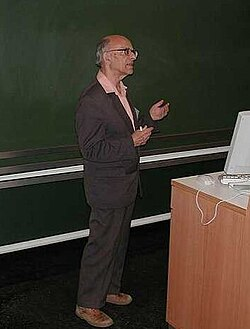
\includegraphics[height=.3\textheight]{./figures/sobol}\par
        {\tiny I.M. Sobol' \\ (1926--)}
        \vspace{0.7ex}
      \end{minipage} 
      \begin{minipage}[b]{0.3\linewidth}
        \centering
        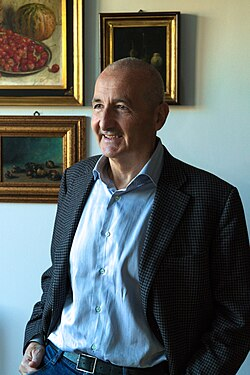
\includegraphics[height=.3\textheight]{./figures/saltelli}\par
        {\tiny A. Saltelli \\ (1953--)} 
      \end{minipage}%% 
      \begin{minipage}[b]{0.3\linewidth}
        \centering
        
\includegraphics[height=.3\textheight]{./figures/owen}\par 
        {\tiny A. Owen \\ (1958--)}
      \end{minipage} 
    \end{figure}
    \vspace{-0.5em}
    {\hfill \raggedright \tiny Credit: Wikipedia, CC-BY-SA-2.0}

  \end{column}
\end{columns}

\end{frame}

%%%%%%%%%%%%%%%%%%%%%%%%%%%%%%%%%%%%%%%%%%%%%%%%%%
\section{Applications}
%%%%%%%%%%%%%%%%%%%%%%%%%%%%%%%%%%%%%%%%%%%%%%%%%%

%=============================================================================
\begin{frame}{Outline}
  \tableofcontents[currentsection]
\end{frame}

%==============================================================================
\begin{frame}[fragile]{Applications and Interpretations}
\small

Given the variance decomposition of $f$ into a sum of \emph{partial variances}:
\begin{equation*}
  \sigma^2 = \sum_{\lvert \bm{u} \rvert > 0} \sigma_{\bm{u}}^2,
\end{equation*}

\begin{exampleblock}{}
  \centering
  We gain insight into $f$ (with respect to its inputs) by \emph{aggregating}
  partial variances into few interpretable numbers.    
\end{exampleblock}

\end{frame}

%%%%%%%%%%%%%%%%%%%%%%%%%%%%%%%%%%%%%%%%%%%%%%%%%%
\subsection{Application: Global Sensitivity Analysis}
%%%%%%%%%%%%%%%%%%%%%%%%%%%%%%%%%%%%%%%%%%%%%%%%%%

%=============================================================================
\begin{frame}{Outline}
  \tableofcontents[currentsubsection]
\end{frame}

%==============================================================================
\begin{frame}[fragile]{Sensitivity Analysis: Local vs Global}
\small
  
\textit{How variation in the inputs affect the variation in the output
of a complex model}

\begin{exampleblock}{}
We often distinguish \emph{local analysis} (effects of perturbations around a particular instance)
from \emph{global analysis} (variations over all possible instances in the domain).    
\end{exampleblock}

\begin{columns}[T,onlytextwidth]
\begin{column}{0.5\textwidth}
  \begin{center}
    %\includegraphics[width=0.35\textwidth]{./figures/failureProbability}
    \begin{tikzpicture}[scale=0.85]
  
      \def\startx{0}    % lower end of domain
      \def\endx{1}      % upper end of domain
  
      \begin{axis}[
        domain=\startx:\endx,
        xmin=0, xmax=1,
        ymin=0, ymax=1,
        enlargelimits=false,
        axis x line=middle,
        axis y line=middle,
        ticks=none,
        height=5cm,
        width=5cm,
        xlabel={$x_1$},
        ylabel={$x_2$}
      ]
      
      \addplot[color=black,mark=*] coordinates {(0.5,0.5)};
      \addplot[color=black,mark=x] coordinates {(0.5,0.25)};
      \addplot[color=black,mark=x] coordinates {(0.25,0.5)};

      \addplot[gray,thin,smooth] coordinates {(0.5,0.5) (0.5,0.25)};
      \addplot[gray,thin,smooth] coordinates {(0.5,0.5) (0.25,0.5)};

      \end{axis}
  
      \end{tikzpicture}\par
      {\footnotesize Local analysis}
    \end{center}
\end{column}
\begin{column}{0.5\textwidth}
  \begin{center}
    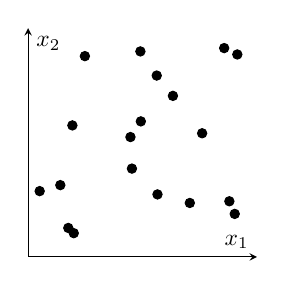
\begin{tikzpicture}[scale=0.85]
  
      \def\startx{0}    % lower end of domain
      \def\endx{1}      % upper end of domain
  
      \begin{axis}[
        domain=\startx:\endx,
        xmin=0, xmax=\endx,
        ymin=0, ymax=\endx,
        enlargelimits=false,
        axis x line=middle,
        axis y line=middle,
        ticks=none,
        height=5cm,
        width=5cm,
        xlabel={$x_1$},
        ylabel={$x_2$},
        scatter/classes={a={mark=*,draw=black}}
      ]
      
      \addplot[scatter src=explicit symbolic,only marks] coordinates {
                                      (0.5620,    0.7928)
                                      (0.4906,    0.8983)
                                      (0.8795,    0.2433)
                                      (0.7066,    0.2359)
                                      (0.1994,    0.1039)
                                      (0.9142,    0.8850)
                                      (0.1933,    0.5749)
                                      (0.8568,    0.9128)
                                      (0.1406,    0.3139)
                                      (0.4472,    0.5240)
                                      (0.7605,    0.5405)
                                      (0.1755,    0.1267)
                                      (0.4925,    0.5925)
                                      (0.6328,    0.7040)
                                      (0.9029,    0.1881)
                                      (0.2480,    0.8777)
                                      (0.0504,    0.2877)
                                      (0.5653,    0.2733)
                                      (0.4536,    0.3861)};
      \end{axis}
  
      \end{tikzpicture}\par
      {\footnotesize Global analysis}
    \end{center}
  \end{column}
\end{columns}

\end{frame}

% %==============================================================================
% \begin{frame}[fragile]{Closed Effect Partial Variances}
% \small

% To interpret the decomposition, we aggregate the partial variances (also called \emph{effects})
% into few interpretable values.

% \vspace{1.0em}

% \textbf{Closed effect} of $\bm{x}_{\bm{u}}$:
% \begin{equation*}
%   \underline{\tau}_{\bm{u}}^2 = \sum_{\bm{v} \subseteq \bm{u}} \sigma^2_{\bm{v}}.
% \end{equation*}
% \begin{exampleblock}{}
%   This effect measures the importance of $\bm{x}_{\bm{u}}$ on $f$ by measuring the \emph{variance of $f$ explained}
%   by the main effects of and interactions within $\bm{x}_{\bm{u}}$, but limited only to $\bm{x}_{\bm{u}}$
%   \textbf{not} with $\sim \bm{u}$.
% \end{exampleblock}

% \vspace{1.0em}

% \textbf{Example}: For $\bm{u} = \{ 1, 2 \}$
% \begin{equation*}
%   \underline{\tau}_{\{ 1, 2 \}}^2 = \sum_{\bm{v} \subseteq \{1, 2 \}} \sigma^2_{\bm{v}} = \sigma^2_{\{1\}} + \sigma^2_{\{2\}} + \sigma^2_{\{1,2\}}.
% \end{equation*}

% \end{frame}

%==============================================================================
\begin{frame}[fragile]{Sobol' Sensitivity Indices: Main Effect}
\small
  
The \emph{Sobol' main-effect index} is defined as the \emph{main-effect partial variance}
of $x_j$ normalized by the total variance:
\begin{equation*}
  S_j \equiv \frac{\sigma^2_{\{j\}}}{\sigma^2}.
\end{equation*}
{\hfill \raggedright \tiny \textcolor{blue}{(\cite{Sobol1993})}}

\vspace{-0.75em}

\begin{exampleblock}{}
  \centering
  This index measures the proportion of the total variance of $f$
  that can be explained \emph{only by} $x_j$
  without any interactions with any other variables.
\end{exampleblock}

\begin{onlyenv}<2>
  \emph{Additive function}: Function with  
  \begin{equation*}
    \sum_{j = 1}^m S_j = 1.0
  \end{equation*}
  is called additive function, i.e.,
  \begin{equation*}
    f(\bm{x}) = f_\emptyset + \sum_{j = 1}^m f_{\{ j \}} (x_j).
  \end{equation*}    
\end{onlyenv}

\end{frame}
  
% %==============================================================================
% \begin{frame}[fragile]{Closed Effect: Sobol' Indices}
% \small

% \textbf{Closed Sobol' index} of $\bm{x}_{\bm{u}}$ is obtained by normalizing the effect by the total variance:
% \begin{equation*}
%   S_{\bm{u}} \equiv \frac{\underline{\tau}_{\bm{u}}^2}{\sigma^2}.
% \end{equation*}

% \vspace{1.0em}

% \textbf{Sobol' main-effect index} is the closed Sobol' index for singletons:
% \begin{equation*}
%   S_j = \frac{\underline{\tau}_{j}^2}{\sigma^2} = \frac{\sigma^2_{\{j\}}}{\sigma^2}.
% \end{equation*}

% \begin{exampleblock}{}
% This index measures the proportion of the total variance of $f$
% that can be explained only by $x_j$ without any interactions with another variable;
% $S_j$ is a \textbf{global sensitivity measure}.

% \vspace{0.5em}
% \end{exampleblock}

% \end{frame}

% %==============================================================================
% \begin{frame}[fragile]{Total Effect}
% \small

% \vspace{1.0em}

% \textbf{Total effect} of $\bm{x}_{\bm{u}}$:
% \begin{equation*}
%   \bar{\tau}_{\bm{u}}^2 = \sum_{\bm{v}: \bm{v} \cap \bm{u} \neq \emptyset} \sigma^2_{\bm{v}}.
% \end{equation*}
% \begin{exampleblock}{}
%   This effect measures the importance of $\bm{x}_{\bm{u}}$ on $f$ by measuring the \emph{variance of $f$ explained}
%   by the main effects and any interactions of variables in $\bm{x}_{\bm{u}}$.
% \end{exampleblock}

% \vspace{1.0em}

% \textbf{Example}: For $\bm{u} = \{ 1, 2 \}$ with $m = 3$:
% \begin{equation*}
%   \bar{\tau}_{\{ 1, 2 \}}^2 = \sum_{\bm{v}: \bm{v} \cap [1:m]} \sigma^2_{\bm{v}} = \sigma^2_{\{1\}} + \sigma^2_{\{2\}} + \sigma^2_{\{1, 2\}} + \sigma^2_{\{1, 3\}} + \sigma^2_{\{2, 3\}} + \sigma^2_{\{1, 2, 3\}}.
% \end{equation*}

% \end{frame}

%==============================================================================
\begin{frame}[fragile]{Sobol' Sensitivity Indices: Total Effect}
\small

The \emph{Sobol' total-effect index} is defined as the \emph{total-effect partial variance}
of $x_j$ normalized by the total variance:
\begin{equation*}
  ST_j \equiv \frac{\bar{\tau}_{\{j\}}^2}{\sigma^2};\;\; \bar{\tau}_{\{j\}}^2 \equiv \sum_{\bm{v}: \bm{v} \cap \{j\} \neq \emptyset} \sigma^2_{\bm{v}}.
\end{equation*}
{\hfill \raggedright \tiny \textcolor{blue}{(\cite{Homma1996})}}

\vspace{1.0em}

\begin{exampleblock}{}
\centering
This index measures the proportion of the total variance of $f$
that can be explained by $x_j$ \emph{and} its interaction with any other variables.
\end{exampleblock}

\vspace{0.5em}

\emph{Example}: For $\{ j \} = \{ 1 \}$ with $m = 3$:
\begin{equation*}
  \bar{\tau}_{\{ 1 \}}^2 = \sum_{\bm{v}: \bm{v} \cap \{ j \} \neq \emptyset} \sigma^2_{\bm{v}} = \sigma^2_{\{1\}} + \sigma^2_{\{1, 2\}} + \sigma^2_{\{1, 3\}} + \sigma^2_{\{1, 2, 3\}}.
\end{equation*}

\end{frame}

%==============================================================================
\begin{frame}[fragile]{Sobol' Sensitivity Indices: Some Interpretations}
\small

Consider the following two cases:

\vspace{1.0em}

\begin{itemize}
  \item $S_j$ is large $\rightarrow$ $x_j$ is important: $S_j$ is a measure of a variable \emph{importance}
  
  \begin{exampleblock}{}
    \centering
    Setting $x_j$ to a particular value (thus reducing its variance to zero) will on average reduce the variance of $f$
    significantly.      
  \end{exampleblock}

  \item $ST_j$ is small $\leftrightarrow$ $x_j$ is not important: $ST_j$ is a measure of a variable \emph{non-importance}

  \begin{exampleblock}{}
    \centering
    Setting $x_j$ to a particular value (thus reducing its variance to zero) will on average do nothing to the variance of $f$.
    $x_j$ doesn't matter.
  \end{exampleblock}

\end{itemize}

\end{frame}

%==============================================================================
\begin{frame}[fragile]{Example: Simple Portfolio Model}
\small

\begin{columns}[T,onlytextwidth]
  \begin{column}{0.6\textwidth}
Consider the following $3$-dimensional function:
\begin{onlyenv}<1>
  \begin{equation*}
    f(\bm{x}) = \blacksquare
  \end{equation*}    
\end{onlyenv}
\begin{onlyenv}<2>
  \begin{equation*}
    f(\bm{x}) = 500 x_1 + 400 x_2 + 100 x_3
  \end{equation*}    
  {\hfill \raggedright \tiny \textcolor{blue}{(\cite{Saltelli2004})}}
\end{onlyenv}

\begin{table}
  \centering
  \vspace{0.5em}
  \begin{tabular}{c c c c} \hline
    Input   & $\rho_X$ & $S_j$ & $ST_j$ \\ \hline
    
    $X_1$   &
    $\mathcal{N}(0.0, 4.0)$ &
    \tikz[baseline]{\node[fill=lightgray,anchor=base] {$0.861$};} & 
    $0.861$ \\

    $X_2$ &
    $\mathcal{N}(0.0, 2.0)$ &
    $0.1376$ &
    $0.1376$ \\

    $X_3$ &
    $\mathcal{N}(0.0, 1.0)$ &
    $0.0021$ &
    \tikz[baseline]{\node[fill=lightgray!60,anchor=base] {$0.0021$};} \\

    \hline
  \end{tabular}    
\end{table}

\vspace{0.5em}

$X_1$ is the most influential input; $X_3$ is the non-influential input; $f$ is additive.

\end{column}

\begin{column}{0.4\textwidth}
  \begin{figure}
    \centering
    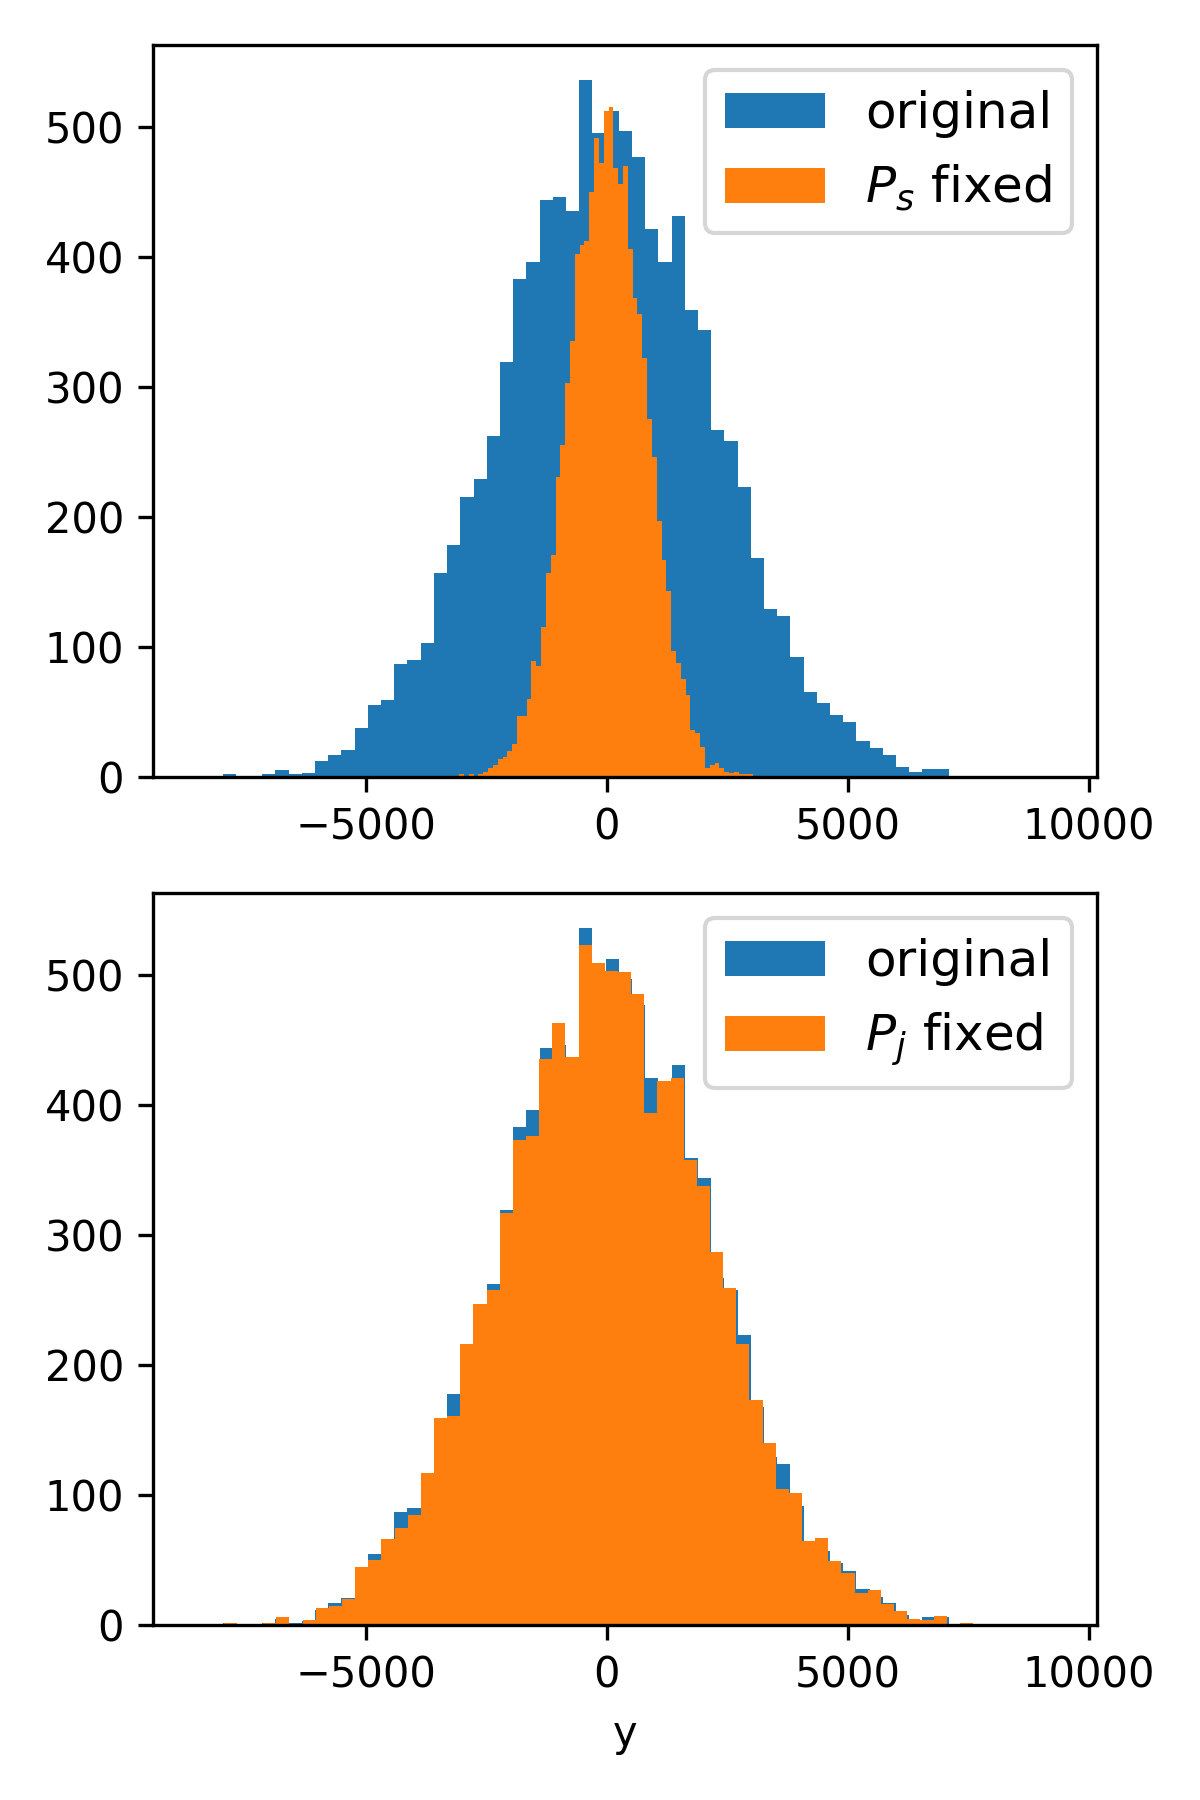
\includegraphics[width=0.7\textwidth]{./figures/portfolio.png}
  \end{figure}
\end{column}

\end{columns}

\end{frame}

%==============================================================================
\begin{frame}[fragile]{Example: Ishigami Function}
  \small
  
  \begin{columns}[T,onlytextwidth]
    \begin{column}{0.6\textwidth}
  Consider the following $3$-dimensional function:
  \begin{onlyenv}<1>
    \begin{equation*}
      f(\bm{x}) = \blacksquare
    \end{equation*}      
  \end{onlyenv}
  
  \begin{onlyenv}<2>
    \begin{equation*}
      f(\bm{x}) = \sin{(x_1)} + 7 \sin{(x_2)}^2 + 0.1 x_3^4 \sin{(x_1)}
    \end{equation*}
    {\hfill \raggedright \tiny \textcolor{blue}{(\cite{Ishigami1991})}}
  \end{onlyenv}


  \begin{table}
    \centering
    \vspace{0.5em}
    \begin{tabular}{c c c c} \hline
      Input   & $\rho_X$ & $S_j$ & $ST_j$ \\ \hline
      
      $X_1$   &
      $\mathcal{U}(-\pi, \pi)$ &
      $0.314$ & 
      $0.558$ \\
  
      $X_2$ &
      $\mathcal{U}(-\pi, \pi)$ &
      \tikz[baseline]{\node[fill=lightgray,anchor=base] {$0.442$};} &
      $0.442$ \\
  
      $X_3$ &
      $\mathcal{U}(-\pi, \pi)$ &
      $0.000$ &
      $0.244$ \\
      \hline
    \end{tabular}    
  \end{table}
  
  \vspace{0.5em}
  
  $X_2$ is the most influential input; no input is non-influential; $f$ is not additive.
  
  \end{column}
  
  \begin{column}{0.4\textwidth}
    \begin{figure}
      \centering
      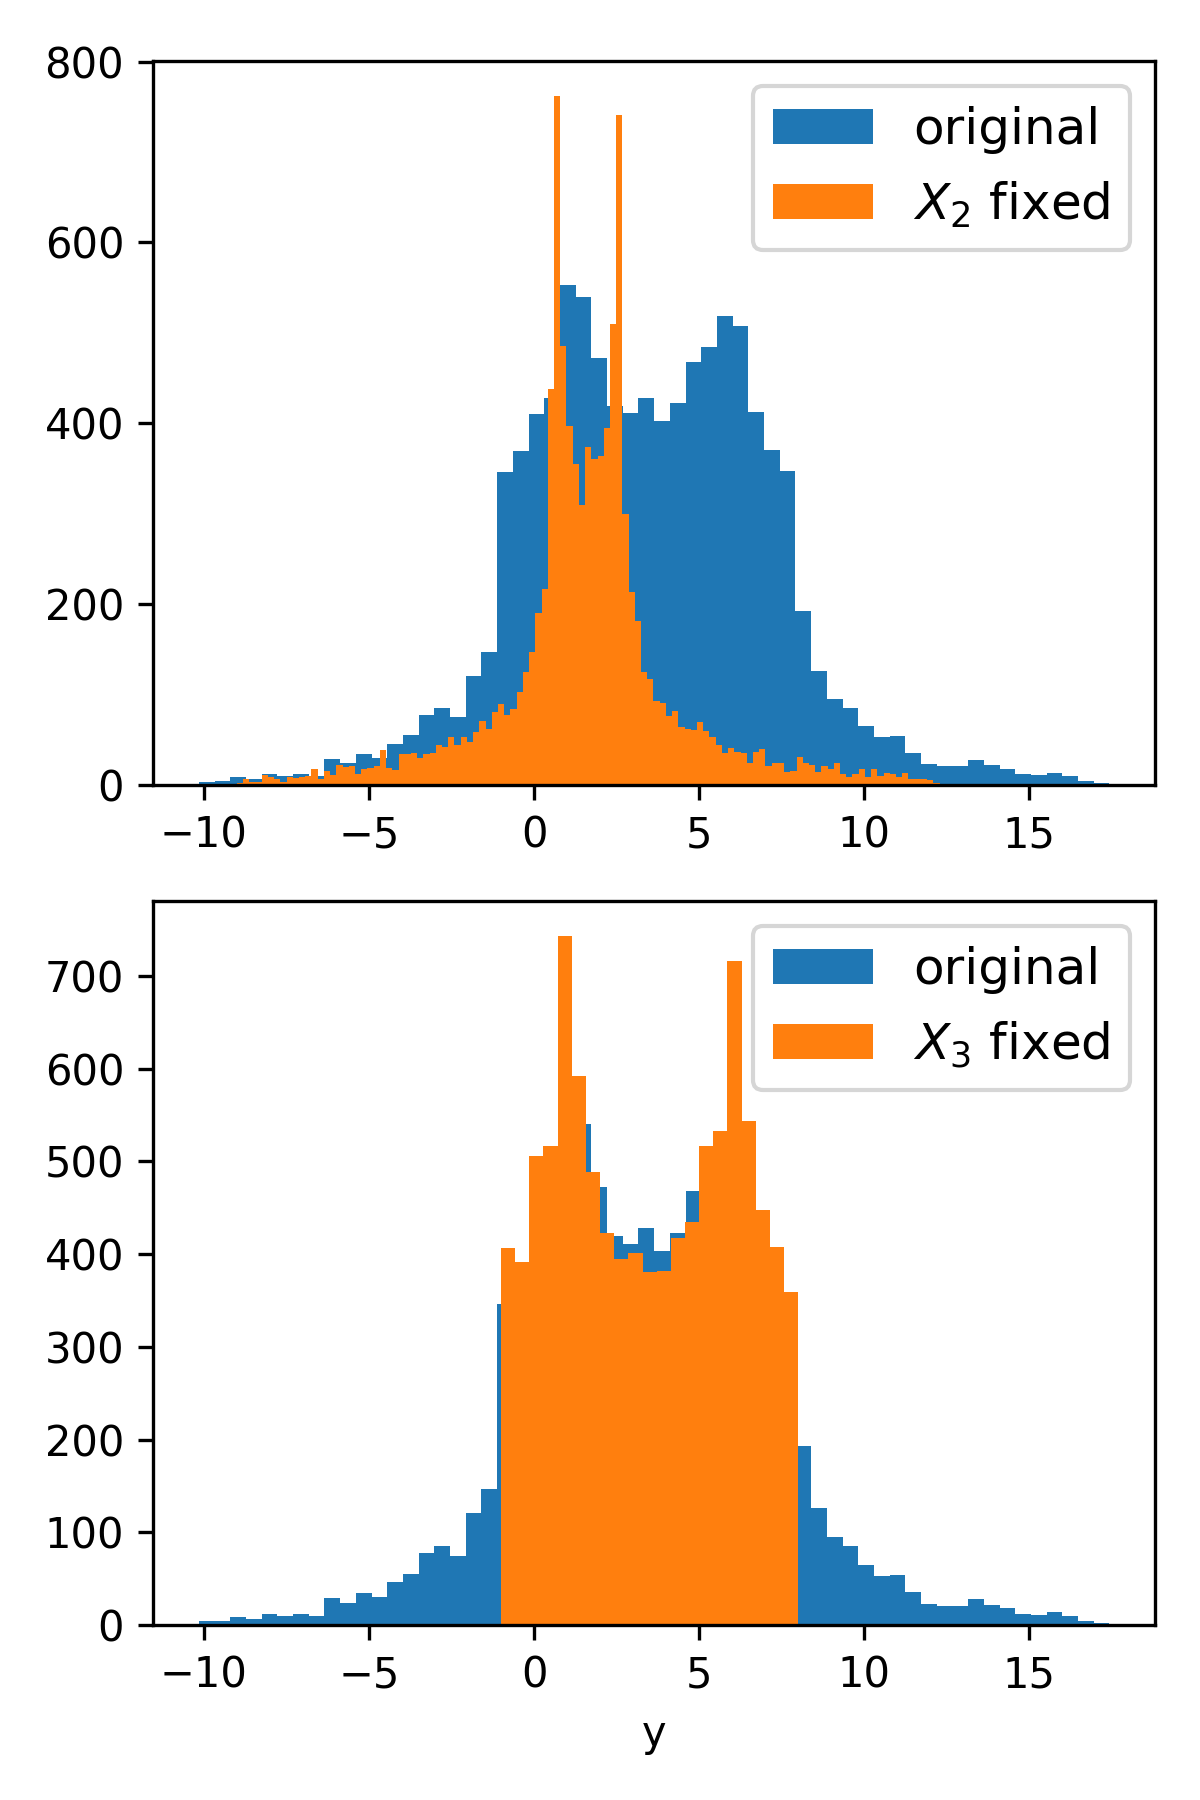
\includegraphics[width=0.7\textwidth]{./figures/ishigami.png}
    \end{figure}
  \end{column}
  
  \end{columns}
  
\end{frame}

%%%%%%%%%%%%%%%%%%%%%%%%%%%%%%%%%%%%%%%%%%%%%%%%%%
\subsection{Application: Effective Dimensions}
%%%%%%%%%%%%%%%%%%%%%%%%%%%%%%%%%%%%%%%%%%%%%%%%%%

%=============================================================================
\begin{frame}{Outline}
  \tableofcontents[currentsubsection]
\end{frame}

%==============================================================================
\begin{frame}[fragile]{Dimensions of Functions: Nominal vs Effective}
\small

Sobol' indices describe function in few numbers;
we can go one step further to characterize functions...

\vspace{1.0em}

The \emph{nominal dimension} of a function is usually known
in advance, but functions often have a lower \emph{effective dimension} 
than their nominal value.

\end{frame}

%==============================================================================
\begin{frame}[fragile]{Effective Dimension: Superposition Sense}
\small

The effective dimension of $f$ in the \emph{superposition sense}
is the smallest integer $m_s$ such that
\begin{equation*}
  \sum_{\lvert \bm{u} \rvert \leq m_s} \sigma_{\bm{u}}^2 \geq p \; \sigma^2,  
\end{equation*}
{\hfill \raggedright \tiny \textcolor{blue}{(\cite{Caflisch1997})}}

where $0 < p < 1$. The choice of $p$ is arbitrary,
but a common choice for $p$ is $0.99$.

\begin{exampleblock}{}
  \centering
  The effective dimension in superposition sense is the \emph{maximum order of interactions}
  one must include in the sum in order to reach the target variance.
\end{exampleblock}

\vspace{0.5em}

For $m_s = 1$, the function is purely \emph{additive}.

\end{frame}

%==============================================================================
\begin{frame}[fragile]{Effective Dimension: Truncation Sense}
\small

The effective dimension of $f$ in the \emph{truncation sense}
is the smallest integer $m_t$ such that
\begin{equation*}
  \sum_{\bm{u} \subseteq [1:m_t]} \sigma_{\bm{u}}^2 \geq p \; \sigma^2.  
\end{equation*}
{\hfill \raggedright \tiny \textcolor{blue}{(\cite{Caflisch1997})}}

where $0 < p < 1$. The choice of $p$ is arbitrary, but a common choice for $p$ is $0.99$.
Here we assumed that we order the first $m_t$ variables with respect to their importance.

\begin{exampleblock}{}
  \centering
  The effective dimension in truncation sense is the number of \emph{active input variables}
  of the function.
\end{exampleblock}

\end{frame}

%==============================================================================
\begin{frame}[fragile]{Example: Simple Portfolio Model}
\small
  

\begin{columns}[T,onlytextwidth]
  \begin{column}{0.6\textwidth}
Consider the following $3$-dimensional function:
\begin{equation*}
  f(\bm{x}) = 500 P_s + 400 P_t + 100 P_j
\end{equation*}
{\hfill \raggedright \tiny \textcolor{blue}{(\cite{Saltelli2004})}}

\begin{table}
  \centering
  \vspace{0.5em}
  \begin{tabular}{c c c c} \hline
    Input   & $\rho_X$ & $S_j$ & $ST_j$ \\ \hline
    
    $X_1$   &
    $\mathcal{N}(0.0, 4.0)$ &
    \tikz[baseline]{\node[fill=lightgray,anchor=base] {$0.861$};} & 
    $0.861$ \\

    $X_2$ &
    $\mathcal{N}(0.0, 2.0)$ &
    $0.1376$ &
    $0.1376$ \\

    $X_3$ &
    $\mathcal{N}(0.0, 1.0)$ &
    $0.0021$ &
    \tikz[baseline]{\node[fill=lightgray!60,anchor=base] {$0.0021$};} \\

    \hline
  \end{tabular}    
\end{table}

\vspace{0.5em}

The effective dimensionalities of this nominally 3D function:
\vspace{0.5em}
\begin{itemize}
  \item $m_s = 1$: Additive function, no interaction
  \item $m_t = 2$: One fewer than the nominal dimension
\end{itemize}

\end{column}

\begin{column}{0.4\textwidth}
  \begin{figure}
    \centering
    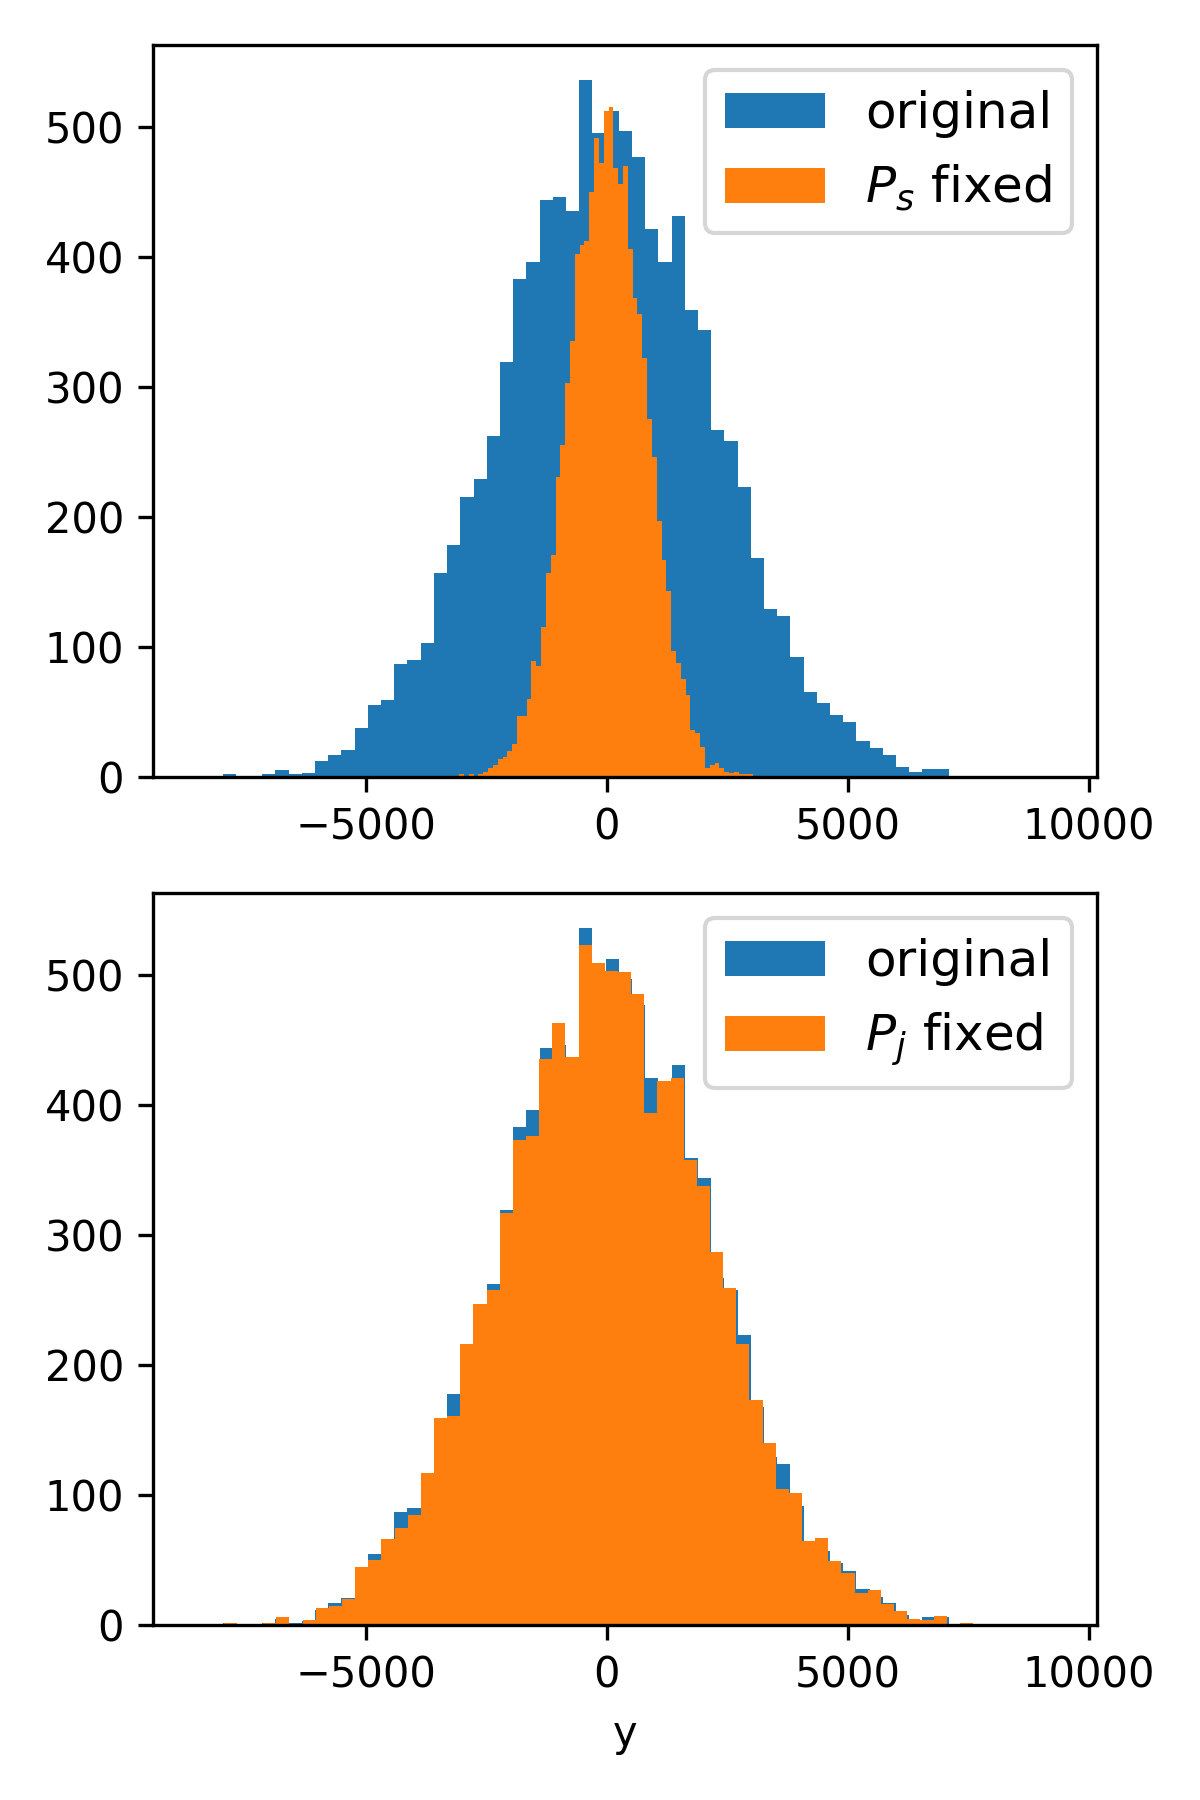
\includegraphics[width=0.7\textwidth]{./figures/portfolio.png}
  \end{figure}
\end{column}

\end{columns}
  
\end{frame}

%==============================================================================
\begin{frame}[fragile]{Example: Ishigami Function}
\small
  
\begin{columns}[T,onlytextwidth]
  \begin{column}{0.6\textwidth}
Consider the following $3$-dimensional function:
\begin{equation*}
  f(\bm{x}) = \sin{(x_1)} + 7 \sin{(x_2)}^2 + 0.1 x_3^4 \sin{(x_1)}
\end{equation*}
{\hfill \raggedright \tiny \textcolor{blue}{(\cite{Ishigami1991})}}

\begin{table}
  \centering
  \vspace{0.5em}
  \begin{tabular}{c c c c} \hline
    Input   & $\rho_X$ & $S_j$ & $ST_j$ \\ \hline
    
    $X_1$   &
    $\mathcal{U}(-\pi, \pi)$ &
    $0.314$ & 
    $0.558$ \\

    $X_2$ &
    $\mathcal{U}(-\pi, \pi)$ &
    \tikz[baseline]{\node[fill=lightgray,anchor=base] {$0.442$};} &
    $0.442$ \\

    $X_3$ &
    $\mathcal{U}(-\pi, \pi)$ &
    $0.000$ &
    $0.244$ \\
    \hline
  \end{tabular}    
\end{table}

\vspace{0.5em}

The effective dimensionalities of this nominally 3D function:
\vspace{0.5em}
\begin{itemize}
  \item $m_s = 2$: Max two-way interaction is required
  \item $m_t = 3$: All inputs are influential
\end{itemize}

\end{column}

\begin{column}{0.4\textwidth}
  \begin{figure}
    \centering
    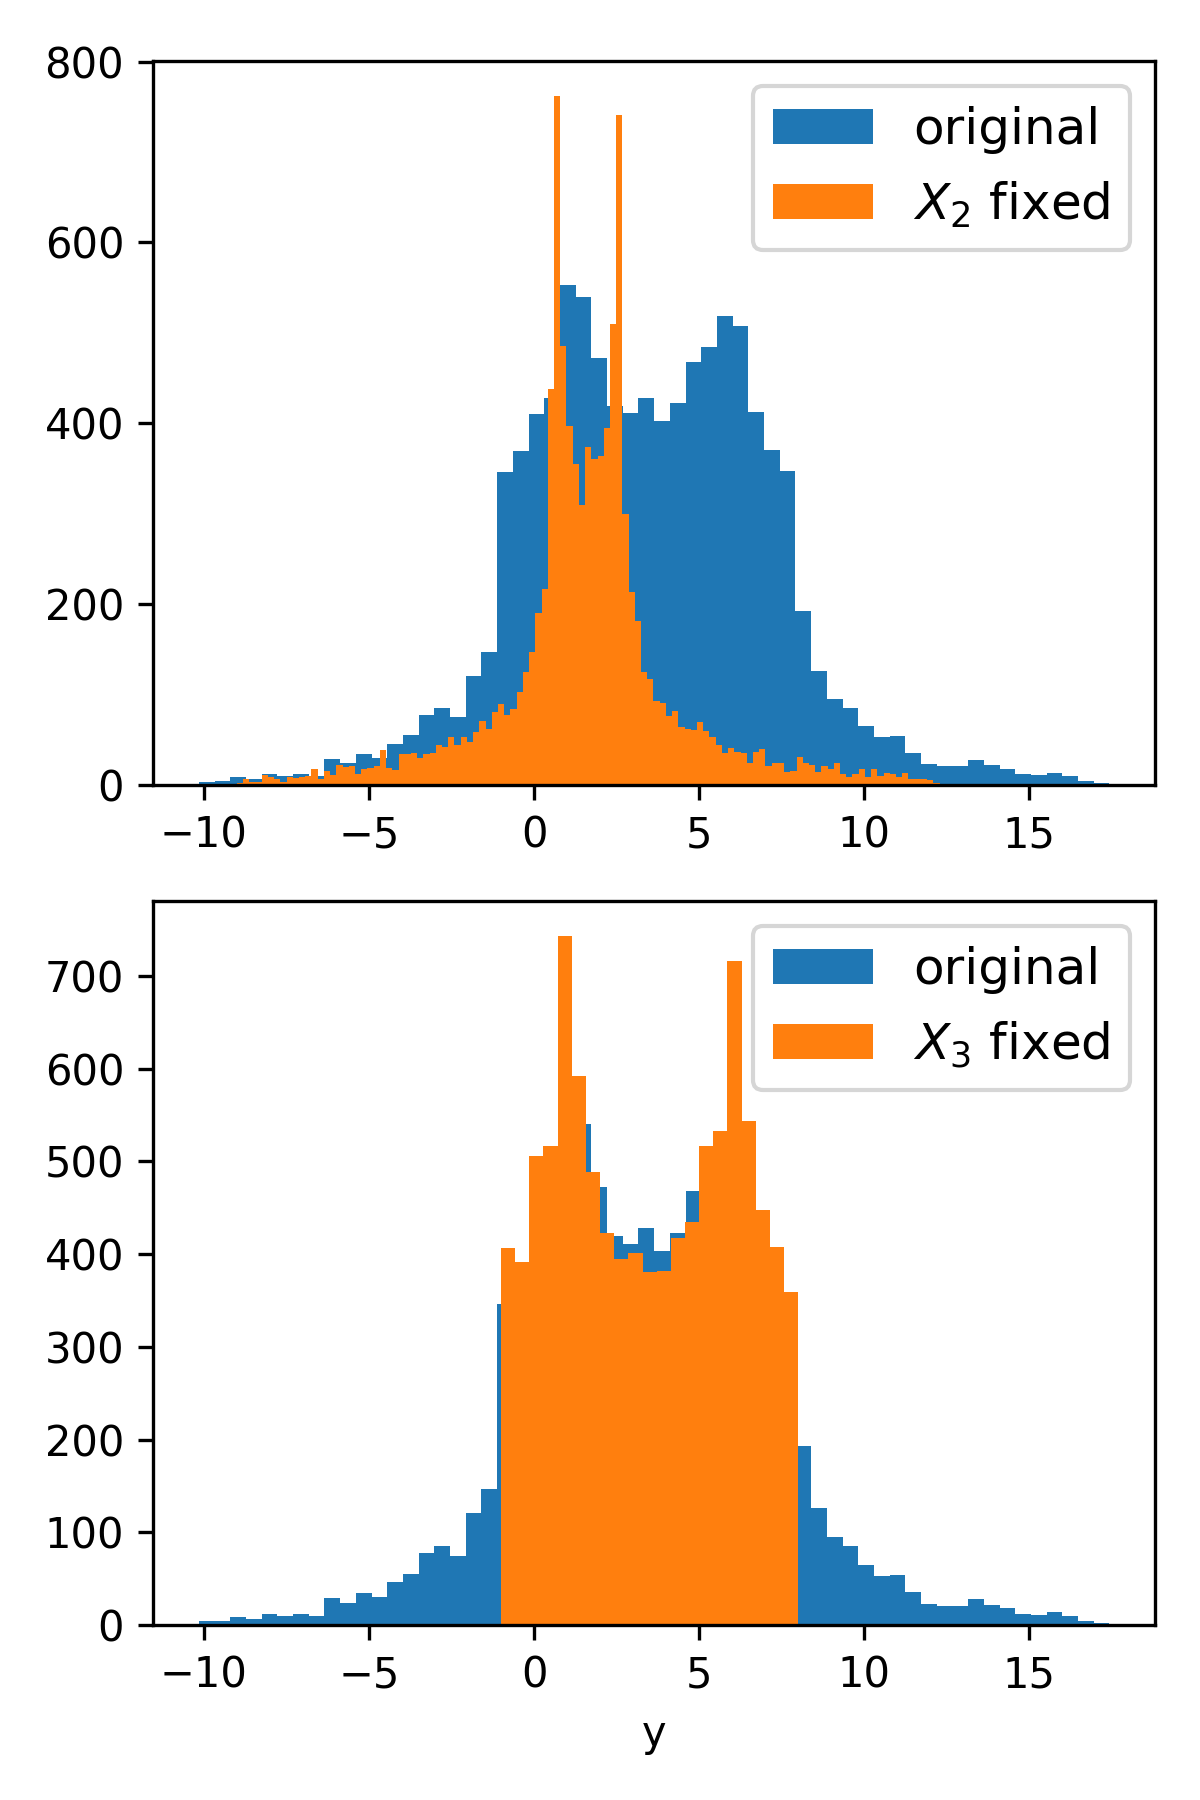
\includegraphics[width=0.7\textwidth]{./figures/ishigami.png}
  \end{figure}
\end{column}

\end{columns}

\end{frame}

%%%%%%%%%%%%%%%%%%%%%%%%%%%%%%%%%%%%%%%%%%%%%%%%%%
\section{Notes on Computation}
%%%%%%%%%%%%%%%%%%%%%%%%%%%%%%%%%%%%%%%%%%%%%%%%%%

%%%%%%%%%%%%%%%%%%%%%%%%%%%%%%%%%%%%%%%%%%%%%%%%%%
\subsection{Notes on Computation: Direct Computation}
%%%%%%%%%%%%%%%%%%%%%%%%%%%%%%%%%%%%%%%%%%%%%%%%%%

%=============================================================================
\begin{frame}{Outline}
  \tableofcontents[currentsubsection]
\end{frame}

%==============================================================================
\begin{frame}[fragile]{Partial Variances: Integration Problems}
\small

\begin{itemize}
  \item To compute the Sobol' main-effect indices, we focus on the following partial variances:
  \begin{equation*}
    \sigma_{\{ j \}}^2 = \int_{\mathcal{D}_{X_{j}}} f^2_{\{j\}} (x_j) \rho_{X_j} (x_j) \; dx_j,\;\; j = 1, \ldots, m.
  \end{equation*}

  \item<2> \only<2>{The following ``\emph{trick}'' often used in probability calculation is useful:
  \begin{equation*}
    \left( \int_{\mathcal{D}_{\bm{X}}} f(\bm{x}) \; d\bm{x} \right)^2 = \int_{\mathcal{D}_{\bm{X}}} f(\bm{x}) \; d\bm{x} \int_{\mathcal{D}_{\bm{X}}} f(\bm{z}) \; d\bm{z},
  \end{equation*}
  where we use a dummy variable $\bm{z}$ to cast the square integrals as a double integral of two independent variables.}

  \item<3-> The following identity can be proven:
  \begin{equation*}
    \sigma_{\{ j \}}^2 = \int\limits_{\mathcal{D}_{\bm{X}_{\sim \{j\}}}} \int\limits_{\mathcal{D}_{\bm{X}}} f(\bm{x}) \; f(x_j, \bm{z}_{\sim \{j\}}) \; \rho_{\bm{X}} (\bm{x}) \; \rho_{\bm{X}_{\sim \{j\}}} (\bm{z}_{\sim \{j\}}) \; d\bm{x} \; d\bm{z}_{\sim \{j\}} - f_\emptyset^2
  \end{equation*}
  where $(x_j, \bm{z}_{\sim \{j\}})$ takes the value of input variables that corresponds
  to the index $j$ from $\bm{x}$ and in $\sim\{j\}$ from $\bm{z}$; $f_\emptyset$ is the mean of $f$ (also an integral).
\end{itemize}

\begin{exampleblock}<4>{}
  \centering
  This is a $(2m - 1)$-fold integral!
\end{exampleblock}

\end{frame}

%==============================================================================
\begin{frame}[fragile]{Partial Variances: Integration Problems}
\small

\begin{itemize}
  \item To compute the Sobol' total-effect indices, we focus on the following partial variances:
  \begin{equation*}
    \bar{\tau}_{\{ j \}}^2 = \sum_{\bm{v}: \bm{v} \cap \{ j \} \neq \emptyset} \sigma_{\bm{v}}^2.
  \end{equation*}

  \item The following identity can be proven:
  \begin{equation*}
    \bar{\tau}_{\{ j \}}^2 = \frac{1}{2} \int\limits_{\mathcal{D}_{X_j}} \int\limits_{\mathcal{D}_{\bm{X}}} \left( f(\bm{x}) - f(z_j, \bm{x}_{\sim \{j\}}) \right) \; \rho_{\bm{X}} (\bm{x}) \; \rho_{X_j} (z_j) \; d\bm{x} \; dz_j,
  \end{equation*}
  where $(z_j, \bm{x}_{\sim \{j\}})$ takes the value of input variables that corresponds
  to the index $j$ from $\bm{z}$ and in $\sim\{j\}$ from $\bm{x}$.
\end{itemize}

\begin{exampleblock}<2>{}
  \centering
  This is an $(m - 1)$-fold integral!
\end{exampleblock}

\end{frame}

%==============================================================================
\begin{frame}[fragile]{Sobol' Indices: Monte Carlo Simulation}
\small

\begin{itemize}
  \item To compute the Sobol' main-effect indices, we cast the integral as expectation:
  \begin{align*}
    \sigma_{\{ j \}}^2 & = \int\limits_{\mathcal{D}_{\bm{X}_{\sim \{j\}}}} \int\limits_{\mathcal{D}_{\bm{X}}} f(\bm{x}) \; f(x_j, \bm{z}_{\sim \{j\}}) \; \rho_{\bm{X}} (\bm{x}) \; \rho_{\bm{X}_{\sim \{j\}}} (\bm{z}_{\sim \{j\}}) \; d\bm{x} \; d\bm{z}_{\sim \{j\}} - f_\emptyset^2 \\
                       & = \mathbb{E}_{\bm{X}, \bm{Z}_{\sim \{ j \}}} \left[ f(\bm{X}) \; f(X_j, \bm{Z}_{\sim \{j\}}) \right] - \mathbb{E}^2_{\bm{X}} [f(\bm{X})]
  \end{align*}
  where $\mathbb{E}_{\cdot}[\cdot]$ is the expectation operator;
  the subscript indicates the random variable with respect to which the expectation is taken.
  
  \item Similarly for the Sobol' total-effect indices:
  \begin{align*}
    \bar{\tau}_{\{ j \}}^2 & = \frac{1}{2} \int\limits_{\mathcal{D}_{X_j}} \int\limits_{\mathcal{D}_{\bm{X}}} \left( f(\bm{x}) - f(z_j, \bm{x}_{\sim \{j\}}) \right) \; \rho_{\bm{X}} (\bm{x}) \; \rho_{X_j} (z_j) \; d\bm{x} \; dz_j \\
                           & = \frac{1}{2} \mathbb{E}_{\bm{X}, Z_j} \left[ \left( f(\bm{X}) - f(Z_j, \bm{X}_{\sim \{j\}}) \right)^2 \right]
  \end{align*}
\end{itemize}

\end{frame}

%==============================================================================
\begin{frame}[fragile]{Sobol' Indices: Monte Carlo Simulation}
  \small

\vspace{-1.25em}
  
Replacing the expectations with sample average:
\begin{align*}
  \sigma_{\{ j \}}^2 & = \mathbb{E}_{\bm{X}, \bm{Z}_{\sim \{ j \}}} \left[ f(\bm{X}) \; f(X_j, \bm{Z}_{\sim \{j\}}) \right] - \mathbb{E}^2_{\bm{X}} [f(\bm{X})] \\ 
  & \approx \frac{1}{N} \sum_{i = 1}^N f(x^{(i)}_j, \bm{x}^{(i)}_{\sim \{j\}}) \; f(x^{(i)}_j, \bm{z}^{(i)}_{\sim \{j}\}) - \left( \frac{1}{N} \sum_{i = 1}^N f(\bm{x}^{(i)}) \right)^2 \\
  \bar{\tau}_{\{ j \}}^2 & = \frac{1}{2} \mathbb{E}_{\bm{X}, Z_j} \left[ \left( f(\bm{X}) - f(Z_j, \bm{X}_{\sim \{j\}}) \right)^2 \right] \\
  & \approx \frac{1}{2N} \sum_{i = 1}^N \left( f(x^{(i)}_j, \bm{x}^{(i)}_{\sim \{j\}}) - f(z^{(i)}_j, \boldsymbol{x}^{(i)}_{\sim \{u\}}) \right)^2 \\
\end{align*}

\vspace{-2.0em}

{\hfill \raggedright \tiny \textcolor{blue}{(\cite{Saltelli2002,Saltelli2010})}}

\vspace{0.25em}

where $\{ \bm{x}^{(i)} \}_{i = 1}^N$ and $\{ \bm{z}^{(i)} \}_{i = 1}^N$ are two independent sets of sample points generated from $\bm{X}$.
The sample variance for normalization can be computed using the same samples.

\vspace{-0.5em}

\begin{exampleblock}<2>{}
  \centering
  Both Sobol' main-effect and total-effect indices for all $m$ variables
  can be computed using $N (m + 2)$ sample points, $N \sim 10^3-10^6$.
\end{exampleblock}

\end{frame}

%%%%%%%%%%%%%%%%%%%%%%%%%%%%%%%%%%%%%%%%%%%%%%%%%%
\subsection{Notes on Computation: Function Approximations}
%%%%%%%%%%%%%%%%%%%%%%%%%%%%%%%%%%%%%%%%%%%%%%%%%%

%=============================================================================
\begin{frame}{Outline}
  \tableofcontents[currentsubsection]
\end{frame}

%==============================================================================
\begin{frame}[fragile]{Polynomial Chaos Expansions}
\small

Alternatively, we can obtain the full functional ANOVA by expanding the random variable $Y = f(\bm{X})$
using orthogonal polynomial basis:
\begin{equation*}
  Y = \sum_{\bm{\alpha} \in \mathbb{N}^m} c_{\bm{\alpha}} \Psi_{\bm{\alpha}} (\bm{X}),\;\; \Psi_{\bm{\alpha}} (\bm{x}) = \prod_{j = 1}^m \psi_j^{(\alpha_j)} (x_j),
\end{equation*}
where:
\begin{itemize}
  \item $\bm{\alpha}$: a multi-index indicating the degree of the polynomial basis in each dimension
  \item $c_{\bm{\alpha}}$: coefficients
  \item $\Psi_{\bm{\alpha}} (\bm{X})$: (multivariate) orthogonal polynomial basis
\end{itemize}

\vspace{0.5em}

From orthogonalities:
\begin{equation*}
  \mathbb{E}\mathbb[\Psi_{\bm{\alpha}} (\bm{X})] = 0;\;\;\; \mathbb{E}\mathbb[\Psi_{\bm{\alpha}} (\bm{X}) \Psi_{\bm{\beta}} (\bm{X})] = \delta_{\bm{\alpha}, \bm{\beta}} 
\end{equation*}

\begin{exampleblock}<2>{}
  \centering
  These properties satisfies all what we need from a functional ANOVA decomposition.
\end{exampleblock}

\end{frame}

%==============================================================================
\begin{frame}[fragile]{Classical orthogonal polynomials}
  \footnotesize
  
  \begin{columns}[T,onlytextwidth]
    \begin{column}{0.70\textwidth}
      \begin{itemize}
        \item Two functions $g$ and $h$ are orthogonal w.r.t $\rho_X$ iff: $\langle g,h \rangle_{\rho_X} = 0$
        \item Several classical orthogonal polynomials are known
              (orthogonality w.r.t classical probability density functions (PDFs))
      \end{itemize}
      \begin{table}
        \centering
      \begin{tabular}{c c c c c} \hline
        Name & Symbol & $\rho_X$ & Support & Distribution  \\ \hline
        & & & & \\
        Legendre & $P^{(p)}(x)$& $\frac{1}{2}$ & $[-1,1]$            & Uniform \\
        & & & & \\
        Hermite  & $He^{(p)}(x)$ & $\frac{1}{\sqrt{2\pi}}e^{-x^2/2}$ & $(-\infty,\infty)$  & Gaussian \\
        & & & & \\
        Laguerre & $La^{(p)}_a(x)$ & $x^a e^{-x}$ & $[0,\infty)$        & Gamma \\
        & & & & \\
        Jacobi   & $J^{(p)}_{a,b}(x)$ & $\frac{(1-x)^\alpha(1+x)^\beta}{B(\alpha+1,\beta+1)}$ & $[-1,1]$             & Beta \\
        \hline
      \end{tabular}
  
      {\hfill \raggedright \tiny \textcolor{blue}{(\cite{Xiu2002})}}
  
      {\hfill \raggedright \tiny Orthonormal polynomials are created by dividing them by the square root of their norm}
  
    \end{table}
  
    \end{column}
    \begin{column}{0.30\textwidth}
      \begin{figure}[ht] 
        \begin{minipage}[b]{0.5\linewidth}
          \centering
          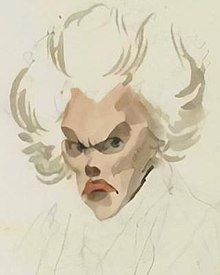
\includegraphics[height=.3\textheight]{./figures/Legendre}\par 
          {\tiny A.-M. Legendre}
          \vspace{0.5ex}
        \end{minipage}%%
        \begin{minipage}[b]{0.5\linewidth}
          \centering
          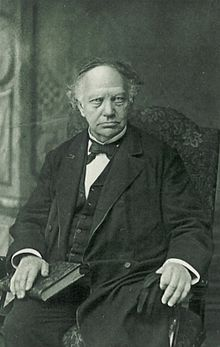
\includegraphics[height=.3\textheight]{./figures/Hermite}\par
          {\tiny C. Hermite}
          \vspace{0.5ex}
        \end{minipage} 
        \begin{minipage}[b]{0.5\linewidth}
          \centering
          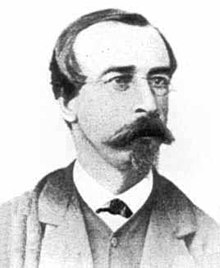
\includegraphics[height=.3\textheight]{./figures/Laguerre}\par
          {\tiny E.N. Laguerre} 
        \end{minipage}%% 
        \begin{minipage}[b]{0.5\linewidth}
          \centering
          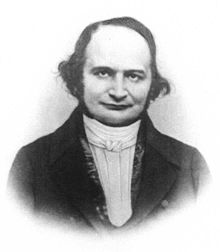
\includegraphics[height=.3\textheight]{./figures/Jacobi}\par 
          {\tiny C.G. Jacobi} 
        \end{minipage} 
      \end{figure}
  
      {\hfill \raggedright \tiny Credit: Wikipedia, CC-BY-SA-2.0}
  
    \end{column}
  \end{columns}
  
  \end{frame}

%==============================================================================
\begin{frame}[fragile]{Polynomial Chaos Expansions: Moments and Partial Variances}
\small

Given PCE, the moments and partial variances of $f$ can be obtained analytically:
\vspace{1em}
\begin{itemize}
  \item \emph{Mean}
  \begin{equation*}
    \mathbb{E}[f(\bm{X})] = c_{\bm{0}}
  \end{equation*}

  \item \emph{Variance}
  \begin{equation*}
    \mathbb{V}[f(\bm{X})] = \sum_{\bm{\alpha} \in \mathbb{N}^M \setminus \{\bm{0}\}} c_{\bm{\alpha}}^2
  \end{equation*}

  \item \emph{Partial variances}
  \begin{equation*}
    \sigma_{\bm{u}}^2 = \sum_{\bm{\alpha} \in A_{\bm{u}}} c_{\bm{\alpha}}^2;\;\;
    A_{\bm{u}} = \{ \bm{\alpha} \in \mathbb{N}^M \setminus \{\bm{0}\}: \alpha_{j \in \bm{u}} \neq 0, \alpha_{j \notin \bm{u}} = 0 \}
  \end{equation*}
\end{itemize}

\begin{exampleblock}<2>{}
  \centering
  Moments and partial variances are combinations of the coefficients of the expansions.
\end{exampleblock}

\end{frame}

%==============================================================================
\begin{frame}[fragile]{Polynomial Chaos Expansions: Sobol' Indices}
\small

Sobol' indices can therefore be obtained analytically:
\vspace{1em}
\begin{itemize}
  \item \emph{Sobol' main-effect indices}
  \begin{equation*}
    \sigma_{\bm{u}}^2 = \frac{\sum_{\bm{\alpha} \in A_{\{j\}}} c_{\bm{\alpha}}^2}{\mathbb{V}[f(\bm{X})]};\;\;
    A_{\{j\}} = \{ \bm{\alpha} \in \mathbb{N}^M \setminus \{\bm{0}\}: \alpha_j \neq 0, \alpha_{i \neq j} = 0  \}
  \end{equation*}

  \item \emph{Sobol' total-effect indices}
  \begin{equation*}
    \sigma_{\bm{u}}^2 = \frac{\sum_{\bm{\alpha} \in \bar{A}_{\{j\}}} c_{\bm{\alpha}}^2}{\mathbb{V}[f(\bm{X})]};\;\;
    \bar{A}_{\{j\}} = \{ \bm{\alpha} \in \mathbb{N}^M \setminus \{\bm{0}\}: \alpha_j \neq 0 \}
  \end{equation*}

  {\hfill \raggedright \tiny \textcolor{blue}{(\cite{Sudret2008})}}

\end{itemize}
  
\end{frame}

%%%%%%%%%%%%%%%%%%%%%%%%%%%%%%%%%%%%%%%%%%%%%%%%%%
\section{Summary}
%%%%%%%%%%%%%%%%%%%%%%%%%%%%%%%%%%%%%%%%%%%%%%%%%%

%=============================================================================
\begin{frame}{Outline}
  \tableofcontents[currentsection]
\end{frame}

%==============================================================================
\begin{frame}[fragile]{Summary}
\small

\begin{itemize}
  \item Functional ANOVA is a valuable tool for the \emph{exploratory analysis} of functions.
  \item Sensitivity measures, such as Sobol' indices,
        provide concise insights into the \emph{importance of input variables}.
  \item Effective dimensions offer an even \emph{more compact characterization} of function
        complexity through a single (or two) numerical value(s).
  \item Monte Carlo estimation and function approximations are two sides of the same coin.
\end{itemize}

\begin{onlyenv}<2>
  \begin{exampleblock}{}
    {``The only way to fight the curse of dimensionality
    is to identify and exploit special structure in the model.''}
  
    {\hfill \raggedright \tiny \textcolor{blue}{(\cite{Constantine2015})}}
  \end{exampleblock}    
\end{onlyenv}

\begin{onlyenv}<3->
  \begin{exampleblock}{}
    {``The only way to fight the curse of dimensionality
    is to \emph{identify} and \emph{exploit} special structure in the model.''}
  
    {\hfill \raggedright \tiny \textcolor{blue}{(\cite{Constantine2015})}}
  \end{exampleblock}    
\end{onlyenv}

\begin{onlyenv}<3->
  {...which can be a bit of a chicken-and-egg problem.}  
\end{onlyenv}

\begin{exampleblock}<4>{}
  \centering
  \textbf{Thank you very much for your attention!}
\end{exampleblock}

\end{frame}

%%%%%%%%%%%%%%%%%%%%%
\appendix
%%%%%%%%%%%%%%%%%%%%%

% %==============================================================================
\begin{frame}[allowframebreaks]{References}
  \printbibliography[heading=none]
\end{frame}

\presentationendframe

\end{document}


%% 
%% Copyright (C) 2019 by Tobias Schlemmer <Tobias.Schlemmer@web.de>
%% 
%% This work may be distributed and/or modified under the
%% conditions of the LaTeX Project Public License (LPPL), either
%% version 1.3c of this license or (at your option) any later
%% version.  The latest version of this license is in the file:
%% 
%% http://www.latex-project.org/lppl.txt
%% 
%% This work is "maintained" (as per LPPL maintenance status) by
%% Tobias Schlemmer.
%% 
%% This work consists of the file CASUS.dtx and a Makefile.
%% Running "make" generates the derived files
%% 
%% • README,
%% • beamerthemeCASUS.pdf,
%% • beamerthemeCASUS.sty,
%% • beamercolorthemeCASUS.sty,
%% • beamerfontthemeCASUS.sty,
%% • beamerinnerthemeCASUS.sty,
%% • beamerouterthemeCASUS.sty,
%% • CASUSbase.sty,
%% • CASUScolors.sty and
%% • minimalexample.tex
%% • demo169.tex
%% 
%% Running "make inst" installs the files in the user's TeX tree.
%% Running "make install" installs the files in the local TeX tree.
%% 
%% The distribution contains graphics files that are subject to their own
%% license.
%% 
%%
%% End of file `minimalexample'.
